% ============================================================================
%  MCKL/manual/manual.tex
% ----------------------------------------------------------------------------
%  MCKL: Monte Carlo Kernel Library
% ----------------------------------------------------------------------------
%  Copyright (c) 2013-2016, Yan Zhou
%  All rights reserved.
%
%  Redistribution and use in source and binary forms, with or without
%  modification, are permitted provided that the following conditions are met:
%
%    Redistributions of source code must retain the above copyright notice,
%    this list of conditions and the following disclaimer.
%
%    Redistributions in binary form must reproduce the above copyright notice,
%    this list of conditions and the following disclaimer in the documentation
%    and/or other materials provided with the distribution.
%
%  THIS SOFTWARE IS PROVIDED BY THE COPYRIGHT HOLDERS AND CONTRIBUTORS "AS IS"
%  AND ANY EXPRESS OR IMPLIED WARRANTIES, INCLUDING, BUT NOT LIMITED TO, THE
%  IMPLIED WARRANTIES OF MERCHANTABILITY AND FITNESS FOR A PARTICULAR PURPOSE
%  ARE DISCLAIMED. IN NO EVENT SHALL THE COPYRIGHT HOLDER OR CONTRIBUTORS BE
%  LIABLE FOR ANY DIRECT, INDIRECT, INCIDENTAL, SPECIAL, EXEMPLARY, OR
%  CONSEQUENTIAL DAMAGES (INCLUDING, BUT NOT LIMITED TO, PROCUREMENT OF
%  SUBSTITUTE GOODS OR SERVICES; LOSS OF USE, DATA, OR PROFITS; OR BUSINESS
%  INTERRUPTION) HOWEVER CAUSED AND ON ANY THEORY OF LIABILITY, WHETHER IN
%  CONTRACT, STRICT LIABILITY, OR TORT (INCLUDING NEGLIGENCE OR OTHERWISE)
%  ARISING IN ANY WAY OUT OF THE USE OF THIS SOFTWARE, EVEN IF ADVISED OF THE
%  POSSIBILITY OF SUCH DAMAGE.
% ============================================================================

\documentclass[
  bib,
  lines=35,
  linespread=1.2,
  fontsize=11pt,
  fontset=Minion,
  monoscale=MatchLowercase,
]{mbook}

\ExplSyntaxOn
\geometry{paperwidth=28\c_mclass_baseline_dim}
\geometry{paperheight=45\c_mclass_baseline_dim}
\ExplSyntaxOff

% ============================================================================
%  MCKL/manual/tex/macro.tex
% ----------------------------------------------------------------------------
%  MCKL: Monte Carlo Kernel Library
% ----------------------------------------------------------------------------
%  Copyright (c) 2013-2016, Yan Zhou
%  All rights reserved.
%
%  Redistribution and use in source and binary forms, with or without
%  modification, are permitted provided that the following conditions are met:
%
%    Redistributions of source code must retain the above copyright notice,
%    this list of conditions and the following disclaimer.
%
%    Redistributions in binary form must reproduce the above copyright notice,
%    this list of conditions and the following disclaimer in the documentation
%    and/or other materials provided with the distribution.
%
%  THIS SOFTWARE IS PROVIDED BY THE COPYRIGHT HOLDERS AND CONTRIBUTORS "AS IS"
%  AND ANY EXPRESS OR IMPLIED WARRANTIES, INCLUDING, BUT NOT LIMITED TO, THE
%  IMPLIED WARRANTIES OF MERCHANTABILITY AND FITNESS FOR A PARTICULAR PURPOSE
%  ARE DISCLAIMED. IN NO EVENT SHALL THE COPYRIGHT HOLDER OR CONTRIBUTORS BE
%  LIABLE FOR ANY DIRECT, INDIRECT, INCIDENTAL, SPECIAL, EXEMPLARY, OR
%  CONSEQUENTIAL DAMAGES (INCLUDING, BUT NOT LIMITED TO, PROCUREMENT OF
%  SUBSTITUTE GOODS OR SERVICES; LOSS OF USE, DATA, OR PROFITS; OR BUSINESS
%  INTERRUPTION) HOWEVER CAUSED AND ON ANY THEORY OF LIABILITY, WHETHER IN
%  CONTRACT, STRICT LIABILITY, OR TORT (INCLUDING NEGLIGENCE OR OTHERWISE)
%  ARISING IN ANY WAY OUT OF THE USE OF THIS SOFTWARE, EVEN IF ADVISED OF THE
%  POSSIBILITY OF SUCH DAMAGE.
% ============================================================================

\addbibresource{manual.bib}

\UseAbbr{aes}
\UseAbbr{ars}
\UseAbbr{avx}
\UseAbbr{blas}
\UseAbbr{brng}
\UseAbbr{cpu}
\UseAbbr{crtp}
\UseAbbr{ess}
\UseAbbr{gcc}
\UseAbbr{gnu}
\UseAbbr{icc}
\UseAbbr{ilp}
\UseAbbr{lapack}
\UseAbbr{llvm}
\UseAbbr{lp}
\UseAbbr{mckl}
\UseAbbr{mcmc}
\UseAbbr{mkl}
\UseAbbr{msvc}
\UseAbbr{pdf}
\UseAbbr{pmf}
\UseAbbr{posix}
\UseAbbr{rdrand}
\UseAbbr{rng}
\UseAbbr{simd}
\UseAbbr{smc}
\UseAbbr{smp}
\UseAbbr{std}
\UseAbbr{stl}
\UseAbbr{tbb}
\UseAbbr{tls}
\UseAbbr{unix}
\UseAbbr{vml}
\UseAbbr{vsl}

\UseAbbr[\aesni][\textsc]{aes-ni}
\UseAbbr[\cpp][\textcase]{C++}
\UseAbbr[\hdf]{hdf5}
\UseAbbr[\ith][\textsups]{t{}h}

\UseMathBB{I}

\UseMathCal{N}
\UseMathCal{X}

\fvset{gobble=2, formatcom=\color{MGrey}}

\def\rmin{r_{\mathrm{min}}}
\def\rmax{r_{\mathrm{max}}}

\def\xobs{X_{\mathrm{obs}}}
\def\xpos{X_{\mathrm{pos}}}
\def\xvel{X_{\mathrm{vel}}}
\def\yobs{Y_{\mathrm{obs}}}
\def\ypos{Y_{\mathrm{pos}}}
\def\yvel{Y_{\mathrm{vel}}}

\tryinput{tex/inc.tex}

\begin{document}

\frontmatter
\title{MCKL}
\subtitle{Monte Carlo Kernel Library}
\author{Yan Zhou}
\date{version 0.1}

\maketitle
\tableofcontents
\listoftables


\mainmatter
% ============================================================================
%  MCKL/manual/tex/introduction.tex
% ----------------------------------------------------------------------------
%  MCKL: Monte Carlo Kernel Library
% ----------------------------------------------------------------------------
%  Copyright (c) 2013-2016, Yan Zhou
%  All rights reserved.
%
%  Redistribution and use in source and binary forms, with or without
%  modification, are permitted provided that the following conditions are met:
%
%    Redistributions of source code must retain the above copyright notice,
%    this list of conditions and the following disclaimer.
%
%    Redistributions in binary form must reproduce the above copyright notice,
%    this list of conditions and the following disclaimer in the documentation
%    and/or other materials provided with the distribution.
%
%  THIS SOFTWARE IS PROVIDED BY THE COPYRIGHT HOLDERS AND CONTRIBUTORS "AS IS"
%  AND ANY EXPRESS OR IMPLIED WARRANTIES, INCLUDING, BUT NOT LIMITED TO, THE
%  IMPLIED WARRANTIES OF MERCHANTABILITY AND FITNESS FOR A PARTICULAR PURPOSE
%  ARE DISCLAIMED. IN NO EVENT SHALL THE COPYRIGHT HOLDER OR CONTRIBUTORS BE
%  LIABLE FOR ANY DIRECT, INDIRECT, INCIDENTAL, SPECIAL, EXEMPLARY, OR
%  CONSEQUENTIAL DAMAGES (INCLUDING, BUT NOT LIMITED TO, PROCUREMENT OF
%  SUBSTITUTE GOODS OR SERVICES; LOSS OF USE, DATA, OR PROFITS; OR BUSINESS
%  INTERRUPTION) HOWEVER CAUSED AND ON ANY THEORY OF LIABILITY, WHETHER IN
%  CONTRACT, STRICT LIABILITY, OR TORT (INCLUDING NEGLIGENCE OR OTHERWISE)
%  ARISING IN ANY WAY OUT OF THE USE OF THIS SOFTWARE, EVEN IF ADVISED OF THE
%  POSSIBILITY OF SUCH DAMAGE.
% ============================================================================

\chapter{Introduction}
\label{chap:Introduction}

\section{Monte Carlo algorithms}
\label{sec:Monte Carlo algorithms}

\section{Using the library}
\label{sec:Using the library}

\subsection{Installation}
\label{sub:Installation}

\subsection{Documents}
\label{sub:Documents}

\section{Organization of headers}
\label{sec:Organization of headers}

\mckl is a header-only library. All headers files are under the "mckl"
directory. To include all functionalities,
\begin{Verbatim}
#include <mckl/mckl.hpp>
\end{Verbatim}
There are a few other headers that include a subset of functions of \mckl, each
documented in a subsequent chapter in this manual. They are listed in
Table~\ref{tab:headers}. These headers does not define anything other than
including other headers that each implement a specific feature. If only one a
few features are needed, then one can include only headers that implement those
features to save compilation time. For example,
\begin{Verbatim}
#include <mckl/random/threefry.hpp>
\end{Verbatim}
includes only the header that implements \rng engines based on the Threefry
algorithm in~\cite{Salmon:2011um} (see Section~\ref{sub:Threefry}). See the
reference manual\footnote{\url{http://zhouyan.github.io/MCKLDoc/master}} for
the header file for each class and function defined in \mckl.

\begin{table}
  \begin{tabularx}{\textwidth}{LL}
    \toprule
    Header & Documents \\
    \midrule
    \texttt{mckl/core.hpp}     & Chapter~\ref{chap:Core concepts}             \\
    \texttt{mckl/smp.hpp}      & Chapter~\ref{chap:Symmetric multiprocessing} \\
    \texttt{mckl/resample.hpp} & Chapter~\ref{chap:Resampling}                \\
    \texttt{mckl/math.hpp}     & Chapter~\ref{chap:Mathemtical functions}     \\
    \texttt{mckl/random.hpp}   & Chapter~\ref{chap:Random number generating}  \\
    \texttt{mckl/random/rng.hpp}
    & Sections~\ref{sec:Counter-based RNG} to~\ref{sec:MKL RNG} \\
    \texttt{mckl/random/distribution.hpp}
    & Section~\ref{sec:Distribution} \\
    \texttt{mckl/random/test.hpp}
    & Section~\ref{sec:Randomness tests} \\
    \texttt{mckl/utility}      & Chapter~\ref{chap:Utilities}                 \\
    \bottomrule
  \end{tabularx}
  \caption{Top-level headers}
  \label{tab:headers}
\end{table}

% ============================================================================
%  MCKL/manual/tex/core.tex
% ----------------------------------------------------------------------------
%  MCKL: Monte Carlo Kernel Library
% ----------------------------------------------------------------------------
%  Copyright (c) 2013-2016, Yan Zhou
%  All rights reserved.
%
%  Redistribution and use in source and binary forms, with or without
%  modification, are permitted provided that the following conditions are met:
%
%    Redistributions of source code must retain the above copyright notice,
%    this list of conditions and the following disclaimer.
%
%    Redistributions in binary form must reproduce the above copyright notice,
%    this list of conditions and the following disclaimer in the documentation
%    and/or other materials provided with the distribution.
%
%  THIS SOFTWARE IS PROVIDED BY THE COPYRIGHT HOLDERS AND CONTRIBUTORS "AS IS"
%  AND ANY EXPRESS OR IMPLIED WARRANTIES, INCLUDING, BUT NOT LIMITED TO, THE
%  IMPLIED WARRANTIES OF MERCHANTABILITY AND FITNESS FOR A PARTICULAR PURPOSE
%  ARE DISCLAIMED. IN NO EVENT SHALL THE COPYRIGHT HOLDER OR CONTRIBUTORS BE
%  LIABLE FOR ANY DIRECT, INDIRECT, INCIDENTAL, SPECIAL, EXEMPLARY, OR
%  CONSEQUENTIAL DAMAGES (INCLUDING, BUT NOT LIMITED TO, PROCUREMENT OF
%  SUBSTITUTE GOODS OR SERVICES; LOSS OF USE, DATA, OR PROFITS; OR BUSINESS
%  INTERRUPTION) HOWEVER CAUSED AND ON ANY THEORY OF LIABILITY, WHETHER IN
%  CONTRACT, STRICT LIABILITY, OR TORT (INCLUDING NEGLIGENCE OR OTHERWISE)
%  ARISING IN ANY WAY OUT OF THE USE OF THIS SOFTWARE, EVEN IF ADVISED OF THE
%  POSSIBILITY OF SUCH DAMAGE.
% ============================================================================

\chapter{Core concepts}
\label{chap:Core concepts}

In this chapter, we introduce the core concepts of the library. There are five
of them. At the center is a user defined class that represents the state space.
It shall contain the state values $X_{1:N_t}^t$. This class may also contain
other members that is specific for the model, such as its data set. Next are
the weights $W_{1:N_t}^t$. These two form the particle system $S_{1:N_t}^t$,
where $S_i^t = (X_i^t,W_i^t)$. A sampler operates on a particle system to
produce samples iteratively. A sampler might also use some monitors to
calculate some estimates $\varphi^t(S_{1:N_t}^t)$ as it progresses. These
concepts are all abstracted in the library. For brevity, in the following we
will drop the time dependent index $t$.

\section{State}
\label{sec:State}

Let $E$ be the state space. A state object represents the states $X_{1:N}$ and
everything it depends on. If there exists an integer $d\ge1$ and some space
$\calX$ such that $E\subseteq\calX^d$. Then, we can represent the states as an
$N$ by $d$ matrix. The element at row $i$ and column $j$ is thus the $j$\ith
component of $X_i$. The library provides a class template to abstract this type
of state space,
\begin{Verbatim}
template <MatrixLayout Layout, size_t Dim, typename ValueType>
class StateMatrix;
\end{Verbatim}
where |Layout| is either |RowMajor| or |ColMajor|, which specifies the matrix
layout, |Dim| is the dimension of $X$, i.e., $d$ and |ValueType| represents
values in $\calX$. For example, if $E\subseteq\Real^d$, then one can use the
following class,
\begin{Verbatim}
StateMatrix<RowMajor, d, double> state(N);
\end{Verbatim}
This is not a general purpose matrix class for use such as linear algebra. It
is more of a container with a few additional methods. Below is some common
operations can be done on |state|,
\begin{Verbatim}
state.size();     // Get sample size
state.dim();      // Get dimension
state.row_size(); // Same as size()
state.col_size(); // Same as dim()
state.resize(N);  // Set sample size
state(i, j);      // The element at row i, column j
state.at(i, j);   // Same as above but with assertion
\end{Verbatim}
If the template parameter |Dim| is equal to zero, then it is assumed that the
dimension is dynamic and may change later. In this case, there is an additional
constructor and other methods,
\begin{Verbatim}
StateMatrix<RowMajor, Dynamic, double> state(N, d);
state.resize(N, d);  // Set sample size and dimension
state.resize_dim(d); // Set dimension
\end{Verbatim}
The enumerator |Dynamic| above has the value zero. Note that, these methods are
only available when the template parameter |Dim| is zero. Attempting to call
these methods when it is positive will result in compile-time errors. Let $p$
be the minimum of the original and new sample sizes, and $q$ be the minimum of
the original and new dimensions. All the methods that change the size of the
matrix will preserve the $p$ by $q$ matrix at the upper left corner of the
original. It is also possible to get pointers to the raw data,
\begin{Verbatim}
state.data();       // &state(0, 0)
state.row_data(i);  // &state(i, 0)
state.col_data(i);  // &state(0, j)
state.row_stride(); // &state(i, j + 1) - &state(i, j)
state.col_stride(); // &state(i + 1, j) - &state(i, j)
\end{Verbatim}
These pointers can provide either read only or read and write access to the raw
data, depends on whether or not the |state| object is constant. Note that, the
strides of the pointers returned by |row_data| and |col_data| depends on the
template parameter |Layout|. To iterate over a specific row,
\begin{Verbatim}
auto rowptr = state.row_data(i);
auto stride = state.row_stride();
auto d = state.dim();
for (size_type j = 0; j != d; ++j, rowptr += stride)
    /* *rowptr is the same as state(i, j) */;
\end{Verbatim}
And similarly, to iterate over a specific column,
\begin{Verbatim}
auto colptr = state.col_data(j);
auto stride = state.col_stride();
auto n = state.size();
for (size_type i = 0; i != n; ++i, colptr += stride)
    /* *colptr is the as state(i, j) */;
\end{Verbatim}
One can also retrieve a whole row or column through an output iterator. For
example, to read the rows~1 and~3 into a vector,
\begin{Verbatim}
std::vector<ValueType> row13(state.dim() * 2);
auto first = row13.begin();
first = state.read_row(1, first);
first = state.read_row(3, first);
\end{Verbatim}
And similarly, to read columns~2 and~4 into a vector,
\begin{Verbatim}
std::vector<ValueType> col24(state.size() * 2);
auto first = col24.begin();
first = state.read_col(2, first);
first = state.read_col(4, first);
\end{Verbatim}
The methods |read_row| and |read_col| return output iterators that point to one
pass the last element in the destination range, similar to that of |std::copy|,
etc. To read the whole matrix into a vector,
\begin{Verbatim}
std::vector<ValueType> mat(state.size() * state.dim());
state.read(RowMajor, mat.begin());
\end{Verbatim}
The first parameter is matrix layout of the output matrix. There are two more
methods, whose purpose will become clear later. The first is,
\begin{Verbatim}
void duplicate(size_type src, size_type dst);
\end{Verbatim}
Let the value of |src| and |dst| be $p$ and $q$, respectively. This method sets
$X^q = X^p$. In other words, $X^p$ is duplicated while $X^q$ is eliminated. The
other method is,
\begin{Verbatim}
template <typename IntType, typename InputIter>
void select(IntType N, InputIter index);
\end{Verbatim}
The first argument is the new sample size, say $\hat{N}$ and |index| is an
$\hat{N}$-vector, say $a_{1:\hat{N}}$. This method selects samples to form a
new collection $\hat{X}_{1:\hat{N}}$  by setting $\hat{X}_i = X_{a_i}$ for $i =
1,\dots,\hat{N}$. The new sample size $\hat{N}$ does not have to be the same as
the original, say $N$. This is closely related to the selection step of \smc
algorithms. Let $r_i = \sum_{j = 1}^{\hat{N}}\bbI_{\{i\}}(a_j)$. Then it is
required that $a_i = i$ for all $r_i > 0$, $i = 1,\dots,\min\{N, \hat{N}\}$.

\section{Weight}
\label{sec:Weight}

The weights $W_{1:N}$ is abstracted by the class |Weight|. For example,
\begin{Verbatim}
Weight w(N);
w.size();    // Get sample size
w.resize(N); // Set sample size
\end{Verbatim}
One important property of |Weight| is that, $W_{1:N}$ is always normalized such
that $\sum_{i=1}^N W_i = 1$. For example, after the construction or resizing,
the weights are set to be equal, i.e., $W_i = 1 / N$, for $i = 1,\dots,N$. This
can also be done manually,
\begin{Verbatim}
w.set_equal();
\end{Verbatim}
The weights can be manipulated in various ways. Let |v| be an input iterator
pointing to an $N$-vector $v_{1:N}$. To set $W_i \propto v_i$,
\begin{Verbatim}
w.set(v);
\end{Verbatim}
To set $ W_i \propto W_i\EE^{v_i}$,
\begin{Verbatim}
w.set_log(v);
\end{Verbatim}
To set weights incrementally, use
\begin{Verbatim}
w.mul(v);
w.add_log(v);
\end{Verbatim}
which set $W_i \propto W_iv_i$ and $W_i \propto W_i \EE^{v_i}$, respectively.
The value of \ess of the weights can be obtained by,
\begin{Verbatim}
w.ess();
\end{Verbatim}
One may also draw an integer $0 \le k < N$ according to the weights by,
\begin{Verbatim}
w.draw(rng);
\end{Verbatim}
where |rng| is a \rng engine object. Last, one can obtain a pointer to the raw
data,
\begin{Verbatim}
w.data();
\end{Verbatim}
or read all the weights into an output iterator,
\begin{Verbatim}
w.read(first);
\end{Verbatim}
Unlike |StateMatrix|, the pointer returned by the |data| method always provides
read only access. In other words, |Weight| does not provide any means for user
to change an individual $W_i$ without changing the others. Conceptually, it is
the relative weights that matter. And changing one of them is in fact changing
$W_{1:N}$ as a whole.

\section{Particle}
\label{sec:Particle}

A particle system, abstracted by the class template,
\begin{Verbatim}
template <typename T>
class Particle;
\end{Verbatim}
is formed by three parts. The first is an object of type |T|, that abstracts
the states $X_{1:N}$. The second is a type |Weight| object that abstracts the
weights $W_{1:N}$. And the third is a collection of \rng engines. There are
some restrictions on the type |T|. The constructor of |Particle| is as the
following,
\begin{Verbatim}
template <typename... Args>
explicit Particle(size_type N, Args &&... args)
\end{Verbatim}
The first argument is the sample size. This and all other arguments, are passed
down to the constructor of type |T|. For example,
\begin{Verbatim}
using T = StateMatrix<RowMajor, Dynamic, double>;
Particle<T> particle(N, d);
\end{Verbatim}
will construct the |StateMatrix| object with arguments |N| and |d|. Therefore,
|T| must has a constructor that accepts an integer value as its first argument.
The additional acceptable arguments of the constructor of |Particle| is the
same as those of |T|. Second, |T| has to provide a |select| method similar to
that of |StateMatrix|. The library does not impose any restriction on the
internal structure of |T|. And thus it cannot perform the selection by itself.
However, for more complicated situations, one can always define a class, say
|ValueType| to represent the space $E$, and use a one dimension |StateMatrix|
as the type |T|. For example,
\begin{Verbatim}
class ValueType; // User defined type
using T = StateMatrix<RowMajor, 1, ValueType>;
Particle<T> particle(N);
\end{Verbatim}
More usefully, one can create a new type by deriving from |StateMatrix|. Note
that, though the |select| method of |StateMatrix| is written as a function
template that can accept any integers and input iterators as its arguments, the
user defined type |T| only needs to support the following signature,
\begin{Verbatim}
ReturnType select(size_type N, const size_type *index);
\end{Verbatim}
where |size_type| is |T::size_type| if such a type exists, and |size_t|
otherwise.

The |Weight| type object is constructed with a single argument, the sample size
$N$. To retrieve references to the type |T| and |Weight| objects, one can call,
\begin{Verbatim}
particle.state();
particle.weight();
\end{Verbatim}
respectively. Last but not least, the |Particle| class also contains a
collection of \rng engines. The method,
\begin{Verbatim}
particle.rng(i);
\end{Verbatim}
returns a reference to an \rng engine, specific to the $i$\ith particle. For $i
\ne j$, if the following,
\begin{Verbatim}
auto &rng_i = particle.rng(i);
auto &rng_j = particle.rng(j);
\end{Verbatim}
are called from two different threads, then |rng_i| and |rng_j| will be
instances of two independent \rng engines. The details are in
Section~\ref{sec:Multiple RNG streams}. The |Particle| class also contains an
\rng engine independent of any particle,
\begin{Verbatim}
auto &rng = particle.rng();
\end{Verbatim}

\subsection{Resize the particle system}
\label{sub:Resize the particle system}

The sample size of a particle system can be obtained by,
\begin{Verbatim}
particle.size();
\end{Verbatim}
It can be changed. However, in Monte Carlo algorithms, one does not change the
sample size arbitrarily. Which samples to be preserved and possibly duplicated
and which samples to be eliminated, has to be done according to some algorithms
that produce desirable effects. There are a few methods to resize a particle
system. They share two common properties. They take the new sample size, say
$M$, as their first argument. The other is that in the end, they call the
|select| method on the type |T| object, with $M$ and an input iterator, say
|index|, that points to an $M$-vector $a_{1:M}$ as arguments. In addition they
all call the |resize| method on the type |Weight| object with $M$ as the
argument. How the type |T| handles the call to the |select| method is up to the
user. But usually it should behave similarly to that of |StateMatrix|. Below is
descriptions of each method for resizing a particle system. They differ in how
they generate the index vector $a_{1:M}$. We will let $N$ denote the original
sample size. Also, for clarity, in the mathematical description of the vectors,
we are using indices starting with $1$, while in the actual program, the
indices starts with zero, as usual.

\subsubsection{Resize with given index vectors}

\begin{Verbatim}
template <typename InputIter>
void resize_by_index(size_type M, InputIter index);
\end{Verbatim}
This method takes the index vector as its input and passes it directly to the
|select| method of |T|.

\subsubsection{Resize with resampling algorithms}

\begin{Verbatim}
template <typename ResampleType>
void resize_by_resample(size_type M, ResampleType &&res)
\end{Verbatim}
This method generates the index vector according to a resampling algorithm. A
resampling algorithm produce the number of replications of each particle in the
original system. The function |res| shall accept a call as the following,
\begin{Verbatim}
res(N, M, rng, w, r);
\end{Verbatim}
where $N$ and $M$ are the original and new sample size, |rng| is a reference to
an \rng engine, |w| is a pointer of type |double|, that points to the
$N$-vector of normalized weights. And last, |r| is a pointer of type
|size_type| that points to the $N$-vector of the number of duplicates of each
particles $r_{1:N}$. It is required that, the results shall satisfy $r_i\ge0$
for $i=1,\dots,N$ and $\sum_{i=1}^N r_i = M$. The index vector is generated
such that,
\begin{gather*}
  a_i = i \text{ if } r_i > 0 \text{ for } i = 1,\dots,\min\{N, M\} \\
  \sum_{i=1}^M\bbI_{\{j\}}(a_i) = r_j \text{ for } j = 1,\dots,N
\end{gather*}

\subsubsection{Resize with uniform selection}

\begin{Verbatim}
void resize_by_uniform(size_type M);
\end{Verbatim}
The index vector is generated such that, $\Prob(a_i = j) = 1/M$, for $i =
1,\dots,M$, $j = 1,\dots,N$. This is equivalent to Multinomial resampling with
equal weights.

\subsection{Clone the particle system}
\label{sub:Clone the particle system}

The |Particle<T>| class has the usual special members, such as the copy
constructor, assignment operator, etc. They work just as usual. For example,
\begin{Verbatim}
auto new_particle = particle;
\end{Verbatim}
This creates a new particle system as an exact duplicate of the original.
However, this ``exactness'' is often undesired. The duplicated particle system
will have exactly the same states of \rng engines as the original. And
therefore, any random samples generated from this new system will be exactly
the same as the original. This is hardly the desired effects in algorithms
where duplicating a particle system into multiple copies is required. In this
situation, one can use the |clone| method,
\begin{Verbatim}
auto new_particle = particle.clone();
\end{Verbatim}
In contrast to the copy constructor, this will create a new particle system
exactly the same as the original, except that all \rng engines within the new
system is re-seeded.

\subsection{Iterate the particle system}
\label{sub:Iterate the particle system}

As mentioned before, the library does not impose restrictions on how the states
shall be structured or accessed. Therefore it is not possible to access $X_i$
using methods of |Particle|. Instead, one has to use methods of |T|, the type
of the template parameter. For example,
\begin{Verbatim}
using T = StateMatrix<RowMajor, d, double>;
Particle<T> particle(N);
particle.state()(i, j);
particle.state().dim();
\end{Verbatim}
This is rather cumbersome and somehow too limited. The library provides a class
template,
\begin{Verbatim}
template <typename T>
class ParticleIndex;
\end{Verbatim}
that represents the index of particles within the system. It is constructed by
the index of the particle and a pointer to the particle system that it belongs
to. For example,
\begin{Verbatim}
ParticleIndex<T> idx(i, &particle);
\end{Verbatim}
or alternatively,
\begin{Verbatim}
auto idx = particle.index(i);
\end{Verbatim}
To access the particle system, use
\begin{Verbatim}
idx.particle();     // A reference to particle
idx.particle_ptr(); // A pointer to particle
\end{Verbatim}
For any type |T|, the type |ParticleIndex<T>| has the following methods,
\begin{Verbatim}
idx.i();   // The index used to construct idx, i
idx.rng(); // => particle.rng(i);
\end{Verbatim}
If |T| is a derived class of |StateMatrix|, then
\begin{Verbatim}
idx.dim();    // => particle.state().dim();
idx.stride(); // => particle.state().row_stride();
idx.data();   // => particle.state().row_data(i);
idx(j);       // => particle.state()(i, j);
idx.at(j);    // => particle.state().at(i, j);
\end{Verbatim}
That is, |ParticleIndex| has an interface that depends on the type |T|. One can
extend its interface by defining a special member class template inside |T|.
For example,
\begin{Verbatim}
using Base = StateMatrix<RowMajor, d, double>;

class T : public Base
{
    public:
    template <typename S>
    using idx_base = Base::particle_index_type<S>;

    template <typename S>
    class particle_index_type : public idx_base<S>
    {
        public:
        particle_index_type(size_type i, Particle<S> *pptr) : idx_base<S>(i, pptr)
        {
        }
    };
};
\end{Verbatim}
The class |ParticleIndex<T>| derives from |T::particle_index_type<T>| if such a
member type exists. Otherwise, it has methods as described earlier for any type
|T|. Therefore, it is possible to give it methods that are more convenient for
a particular problem. We will see examples later in Section~\ref{sec:Example
(PF)}.

The |ParticleIndex| type can also be used like an random access iterator. For
example,
\begin{Verbatim}
auto idx = particle(i);
auto jdx = particle(j);
++idx;      // => particle.index(i + 1);
idx--;      // => particle.index(i - 1);
idx + n;    // => particle.index(i + n);
idx - jdx;  // => i - j;
idx == jdx; // => i == j;
\end{Verbatim}
Other comparison operators such as |!=|, |<|, etc., are also defined. Note
that, comparing or subtracting two indices from two different particles systems
is meaningless. This will result in runtime errors unless debugging is disabled
(see Section~\appref{sec:Error handling}). The increment and decrement
operators follow usual prefix and postfix semantics. However, it is important
to note that, |ParticleIndex| \emph{is not} an iterator even though it shares
many common methods. Recall that, |Particle| does not have methods to access
$X_i$ directly. And therefore it is not possible to dereference a
|ParticleIndex| object to get a reference to $X_i$. Instead, dereferencing an
|ParticleIndex| object will return a reference to itself. This is similar for
the member access operator and the index operator. For example,
\begin{Verbatim}
*idx;       // => idx
idx->rng(); // => idx.rng();
idx[n];     // => idx + n
\end{Verbatim}
These methods may at first seem pointless. However, it makes it possible to
iterate a |Particle| object. For example,
\begin{Verbatim}
for (auto idx : particle) {
    idx(0) = /* initialize the first dimension */;
    idx(1) = /* initialize the second dimension */;
    // ...
}
\end{Verbatim}
This is equivalent to
\begin{Verbatim}
for (size_t i = 0; i != particle.size(); ++i) {
    auto idx = particle.index(i);
    // ...
}
\end{Verbatim}
More importantly, it allows the use of |Particle| with algorithms. For example,
\begin{Verbatim}
auto s = std::accumulate(particle.begin(), particle.end(), 0.0,
    [](double s, ParticleIndex<T> idx) { return s + idx(0); });
\end{Verbatim}

\section{Monitor}
\label{sec:Monitor}

Let $\varphi(S_{1:N})$ be some estimator with values in $\Real^d$. It is often
of interest to monitor its value as the algorithm progresses. In the library,
this is done through the class template |Monitor|. It has the following
constructor,
\begin{Verbatim}
Monitor(
    size_t dim,
    const eval_type &eval,
    bool record_only = false,
    MonitorStage stage = MonitorMCMC);
\end{Verbatim}
The first parameter |dim| is the dimension of $\varphi$, $d$. The second is a
user defined callback function. More specifically,
\begin{Verbatim}
using eval_type = std::function<void(size_t, size_t, Particle<T> &, double *)>;
\end{Verbatim}
For example,
\begin{Verbatim}
void phi(size_t t, size_t d, Particle<T> &particle, double *r);
\end{Verbatim}
When this function is called. The first argument passed to it is $t$, the
iteration number. The second is $d$, the dimension. The third is a reference to
the particle system at iteration $t$. And the last is a pointer to a vector for
output. The third parameter of the constructor, |record_only|, determines how
shall the function above behave. If it is true, then the function |phi| shall
return the value of $\varphi$ directly, and the output parameter |r| points to
a $d$-vector. In this case, |Monitor| merely records the values of $\varphi$ at
each iteration. On the other hand, if |record_only| is false, then it is
assumed that $\varphi$ takes the following form,
\begin{equation*}
  \varphi(X_{1:N}) = \sum_{i=1}^N W_i \varphi_i(X_i).
\end{equation*}
And the output parameter |r| is an $N$ by $d$ row major matrix, with the
$d$-vector value $\varphi_i(X_i)$ written into each row of this matrix. And
each time |phi| is called, |Monitor| will compute and store the result of the
summation above. The last parameter of the constructor of |Monitor| specifies
when shall the calculation of $\varphi$ be carried out. We will defer its
discussion until we introduce the sampler in the next section. The evaluation
object can be replaced later by the following method,
\begin{Verbatim}
void eval(
    const eval_type &e, bool record_only = false, MonitorStage stage = MonitorMCMC);
\end{Verbatim}
One can retrieve the results in various ways. Every time a monitor being
evaluated, it records two values. The first is the iteration number $t$, at
which it was evaluated. The other is the value of $\varphi$. One can retrieve
these values using the following methods,
\begin{Verbatim}
mon.iter_size();  // Total number of evaluations
mon.index(j);     // Iteration number of the j-th evaluation
mon.record(i, j); // The value of the i-th component
                  // of the result at the j-th evaluation
\end{Verbatim}
Note that, the monitor does not have to be added to a sampler before it
starting initialization. It can also be removed before the sampler finishing
all iterations. Therefore, the iteration numbers of a monitor being evaluated
are not necessarily the sequence $0,1,\dots,n$, where $n$ is the total number
of iterations.

\section{Sampler}
\label{sec:Sampler}

\subsection{Construction and configuration}
\label{sec:Construction and configuration}

A sampler is formed by the particle system together with all the operations on
it. It is abstracted by the class template,
\begin{Verbatim}
template <typename T>
class Sampler;
\end{Verbatim}
The template parameter |T| is the same as that of |Particle|. Its constructor
takes arbitrary arguments,
\begin{Verbatim}
template <typename... Args>
explicit Sampler(Args &&... args)
\end{Verbatim}
and all arguments are passed down to the constructor of |Particle|. For
example,
\begin{Verbatim}
using T = StateMatrix<RowMajor, Dynamic, double>;
Sampler<T> sampler(N, d);
\end{Verbatim}
Any callable objects that is convertible to the following can be used as
operations on the particle system,
\begin{Verbatim}
using eval_type = std::function<void(size_t, Particle<T> &)>;
\end{Verbatim}
For example,
\begin{Verbatim}
void eval(size_t iter, Particle<T> &particle);
\end{Verbatim}
Conceptually, such a function implement an operator $M(S_{1:N})$ such that a
new particle system $\hat{S}_{1:\hat{N}}$ is produced given the iteration
number $t$ and the original. It it often possible to decompose the operator $M$
into multiple simpler ones. And thus a sampler can have a sequence of
evaluation objects. Each of these evaluation objects can be added to the
sampler by the |eval| method,
\begin{Verbatim}
Sampler<T> &eval(const eval_type &e, SamplerStage stage);
\end{Verbatim}
For example,
\begin{Verbatim}
sampler.eval(eval, SamplerInit | SamplerMove, true);
\end{Verbatim}
The first argument is the evaluation object. The sampler maintains a sequence
of evaluation steps. The new evaluation object will be appended to the existing
sequence. Note that, the order at which these objects being evaluated is the
same as the one they are added to the sampler. One can clear the sequence by,
\begin{Verbatim}
sampler.eval_clear();
\end{Verbatim}
The second argument will be explained in the next section. The sampler can also
have an optional resampling step. This can be added to the sampler by the
following method,
\begin{Verbatim}
Sampler<T> &resample_method(
    ResampleScheme scheme, double threshold = resample_threshold_always());
\end{Verbatim}
which uses a builtin resampling scheme of the library (see
Section~\ref{sec:Algorithm}). Or alternatively,
\begin{Verbatim}
Sampler<T> &resample_method(
    const eval_type &res_eval, double threshold = resample_threshold_always());
\end{Verbatim}
In either case, the parameter |threshold| specifies the condition under which
the resampling step will be actually performed. Let its value be $\alpha$,
resampling is performed if and only if $\ess < \alpha N$.

Multiple monitors can be added to a sampler. For example,
\begin{Verbatim}
Monitor<T> mon(d, phi, false, MonitorMCMC);
sampler.monitor("name", mon);
\end{Verbatim}
A reference to the named monitor can be retrieved,
\begin{Verbatim}
auto &m = sampler.monitor("name");
\end{Verbatim}

\subsection{Initialization and iteration}
\label{sub:Initialization and iteration}

The sampler can be initialized,
\begin{Verbatim}
sampler.initialize();
\end{Verbatim}
This will perform a few things. First, any record of previous operations on the
sampler will be cleared. The iteration number $t$ will be set to zero. And
then, there are three evaluation stages and three monitoring stages. They are
performed in the following order:

\begin{enumerate}
  \item |SamplerInit|
  \item |MonitorMove|
  \item Resample if $\ess < \alpha N$
  \item |MonitorResample|
  \item |SamplerMCMC|
  \item |MonitorMCMC|
\end{enumerate}

Each evaluation object, added to the sampler through,
\begin{Verbatim}
Sampler<T> &eval(const eval_type &e, SamplerStage stage);
\end{Verbatim}
will be evaluated at the |SamplerInit|, etc., steps if the corresponding stage
is set (i.e., the value of |stage & SamplerInit| is non-zero). Similarly, every
monitor, constructed by,
\begin{Verbatim}
Monitor(
    size_t dim,
    const eval_type &eval,
    bool record_only = false,
    MonitorStage stage = MonitorMCMC);
\end{Verbatim}
will be evaluated if the corresponding stage is the same (e.g., |stage|
\emph{equal} to |MonitorMove|). The sampler can be iterated,
\begin{Verbatim}
sampler.iterate();  // iterate once
sampler.iterate(n); // iterate n times
\end{Verbatim}
At each iteration, the steps performed is the same as initialization, except
that |SamplerInit| is replaced by |SamplerMove|. Therefore, one can distinguish
between operations for initialization or iteration only, and those for every
step. We will see an example in the next section.

\section{Example}
\label{sec:Example (PF)}

This is an example used in \cite{Johansen:2009wd}. Through this example, we
will show how to implement a simple particle filter. It shall walk one through
the basic features of the library introduced above.

\subsection{Model and algorithm}
\label{sub:Model and algorithm}

The state space model, known as the almost constant velocity model in the
tracking literature, provides a simple scenario. The state vector,
\begin{equation*}
  X^t = (\xpos^t, \ypos^t, \xvel^t, \yvel^t)^{\transpose}
\end{equation*}
contains the position and velocity of an object moving in a plane. Imperfect
observations $Y^t = (\xobs^t, \yobs^t)^{\transpose}$ of the positions are
possible at each time instance. The state and observation equations are linear
with additive noises,
\begin{align*}
  X^t &= AX^{t-1} + U^t \\
  Y^t &= BX^t + \delta V^t
\end{align*}
where
\begin{equation*}
  A = \begin{pmatrix}
    1 & 0 & \Delta & 0      \\
    0 & 1 & 0      & \Delta \\
    0 & 0 & 1      & 0      \\
    0 & 0 & 0      & 1
  \end{pmatrix} \qquad
  B = \begin{pmatrix}
    1 & 0 & 0 & 0 \\
    0 & 1 & 0 & 0 \\
  \end{pmatrix} \qquad
  \delta = 0.1
\end{equation*}
and we assume that the elements of the noise vector $U_t$ are independent
Gaussian with variance $0.02$ and $0.001$ for position and velocity,
respectively. The observation noise, $V_t$ comprises i.i.d.\ $t$-distributed
random variables with degree of freedom $\nu = 10$. The prior at time $0$
corresponds to an axis-aligned Gaussian with variance $4$ for the position
coordinates and $1$ for the velocity coordinates. The particle filter algorithm
is shown in Algorithm~\ref{alg:pf}.

\begin{algorithm}[t]
  \begin{algorithmic}
    \tophrule
    \STATE \COMMENT{Initialization}
    \STATE Set $t\leftarrow0$.
    \STATE Sample $\xpos^{0,i},\ypos^{0,i}\sim\calN(0,4)$ and
    $\xvel^{0,i},\yvel^{0,i}\sim\calN(0,1)$.
    \STATE Weight $W_i^0 \propto \exp\{\ell(X_i^0 \vert Y_0)\}$

    \REPEAT
    \STATE \COMMENT{Iteration}
    \STATE Set $t\leftarrow t + 1$.
    \STATE Sample
    \begin{align*}
      \xpos^{t,i}&\sim\calN(\xpos^{t-1,i} + \Delta\xvel^{t-1,i}, 0.02) &
      \xvel^{t,i}&\sim\calN(\xvel^{t-1,i}, 0.001) \\
      \ypos^{t,i}&\sim\calN(\ypos^{t-1,i} + \Delta\yvel^{t-1,i}, 0.02) &
      \yvel^{t,i}&\sim\calN(\yvel^{t-1,i}, 0.001)
    \end{align*}
    \STATE Weight $W_i^t \propto W_i^{t - 1}\exp\{\ell(X_i^t \vert Y_t)\}$.
    \UNTIL{All data are processed}
    \bottomhrule
  \end{algorithmic}
  \caption{Particle filter for the almost constant velocity model}
  \label{alg:pf}
\end{algorithm}

\subsection{Implementation}
\label{sub:Implementation (PF)}

We will work through a complete implementation using a top-down approach.
First, we show the contents |main| function.
\begin{Verbatim}
const size_t N = 1000;
Sampler<PF> sampler(N);

sampler.resample_method(Stratified, 0.5)
    .eval(PFInit, SamplerInit)
    .eval(PFMove, SamplerMove)
    .eval(PFWeight, SamplerInit | SamplerMove)
    .monitor("pos", Monitor<PF>(2, PFEstimate));

sampler.initialize();
sampler.iterate(sampler.particle().state().n() - 1);

std::ofstream out("pf.est");
out << sampler;
out.close();
\end{Verbatim}
Within the |main| function, a |Sampler| object is first constructed with the
specified number of particles. Then we configure the sampler. First, it will
use stratified resampling when $\ess < N / 2$. The sampling step within the
\emph{Initialization} and \emph{Iteration} in Algorithm~\ref{alg:pf} will be
implemented by two functions, |PFInit| and |PFMove|, respectively. The
weighting is done through the function |PFWeight|. And the estimate will be
monitored through the function |PFEstimate|. These are added to the sampler
through the |eval| and |monitor| methods as shown above. It then initialized
and iterated $n - 1$ times, where $n$ is the total number of observations. In
the end, we write a summary of the sampler into the file |pf.est|.

\subsubsection{State}

First all of, we need a class to represent the state space, which is $\Real^4$.
A sensible base class is thus,
\begin{Verbatim}
using PFBase = StateMatrix<RowMajor, 4, double>;
\end{Verbatim}
The class |PF| is declared as below,
\begin{Verbatim}
class PF : public PFBase
{
    public:
    template <typename T>
    class particle_index_type;

    PF(size_t N);
    size_t n() const { return obs_x_.size(); };

    private:
    std::vector<double> obs_x_;
    std::vector<double> obs_y_;
};
\end{Verbatim}
The constructor will initialize the observations,
\begin{Verbatim}
PF(size_t N) : PFBase(N)
{
    double x = 0;
    double y = 0;
    std::ifstream data("pf_cv.data");
    while (data >> x >> y) {
        obs_x_.push_back(x);
        obs_y_.push_back(y);
    }
    data.close();
}
\end{Verbatim}
Again, in a real application, the data is unlikely to be initialized in this
way. The method |n| simply return the size of |obs_x_|. Last, we would like to
extend the |ParticleIndex<PF>| class, by defining a |particle_index_type|
member class template,
\begin{Verbatim}
template <typename T>
using PFIndexBase = PFBase::particle_index_type<T>;

template <typename T>
class particle_index_type : public PFIndexBase<T>
{
    public:
    particle_index_type(size_t i, Particle<T> *pptr) : PFIndexBase<T>(i, pptr)
    {
    }

    double &pos_x() { return this->at(0); }
    double &pos_y() { return this->at(1); }
    double &vel_x() { return this->at(2); }
    double &vel_y() { return this->at(3); }

    double log_likelihood(size_t iter);
};
\end{Verbatim}
First of all, we don't want to later refer to the states $\xpos$, etc., by
integer index values in the reset of the program, which is error prone even for
this simple example. Second, we would like to compute the log-likelihood of any
given particle. This is implemented through the |log_likelihood| method, which
is a simple translation of the mathematical formulation,
\begin{Verbatim}
double log_likelihood(size_t iter)
{
    const double x = this->particle().state().obs_x_[iter];
    const double y = this->particle().state().obs_y_[iter];
    const double scale = 10;
    const double nu = 10;

    double llh_x = scale * (pos_x() - x);
    double llh_y = scale * (pos_y() - y);
    llh_x = std::log(1 + llh_x * llh_x / nu);
    llh_y = std::log(1 + llh_y * llh_y / nu);

    return -0.5 * (nu + 1) * (llh_x + llh_y);
}
\end{Verbatim}

\subsubsection{Initialization and iteration}

The function that sample the state values from the prior is as the following,
\begin{Verbatim}
void PFInit(size_t, Particle<PF> &particle)
{
    const double sd_pos = 2;
    const double sd_vel = 1;
    std::normal_distribution<double> rpos(0, sd_pos);
    std::normal_distribution<double> rvel(0, sd_vel);
    auto &rng = particle.rng();

    for (auto idx : particle) {
        idx.pos_x() = rpos(rng);
        idx.pos_y() = rpos(rng);
        idx.vel_x() = rvel(rng);
        idx.vel_y() = rvel(rng);
    }
}
\end{Verbatim}
We construct two Normal distribution objects using for the position and
velocity components of the states. And initialize each particle with them. The
function to sample new states in each iteration later is similar,
\begin{Verbatim}
void PFMove(size_t, Particle<PF> &particle)
{
    const double sd_pos = std::sqrt(0.02);
    const double sd_vel = std::sqrt(0.001);
    std::normal_distribution<double> rpos(0, sd_pos);
    std::normal_distribution<double> rvel(0, sd_vel);
    auto &rng = particle.rng();
    const double delta = 0.1;

    for (auto idx : particle) {
        idx.pos_x() += rpos(rng) + delta * idx.vel_x();
        idx.pos_y() += rpos(rng) + delta * idx.vel_y();
        idx.vel_x() += rvel(rng);
        idx.vel_y() += rvel(rng);
    }
}
\end{Verbatim}
Both of these two functions are really simple translations of the mathematical
formulation of the algorithm.

\subsubsection{Weighting}

In each iteration, we will weight the particles using its log-likelihood. This
will be computed with the |log_likelihood| method of |particle_index_type|
defined earlier,
\begin{Verbatim}
void PFWeight(size_t iter, Particle<PF> &particle)
{
    std::vector<double> weight(particle.size());
    for (auto idx : particle)
        weight[idx.i()] = idx.log_likelihood(iter);
    particle.weight().add_log(weight.data());
}
\end{Verbatim}
The last step in the function above add the logarithm of the incremental
weights to the particle system. Note that, each time the |initialize| method of
|Sampler| is called, the weights will be set to be equal first. And thus the
function above is correct for both initialization and iterations.

\subsubsection{Estimation}

Last, we would like to record the value of $\varphi^t(X_i^t) =
(\xpos^{t,i},\ypos^{t,i})^{\transpose}$. This is done by defining the function,
\begin{Verbatim}
void PFEstimate(size_t, size_t, Particle<PF> &particle, double *r)
{
    for (auto idx : particle) {
        *r++ = idx.pos_x();
        *r++ = idx.pos_y();
    }
}
\end{Verbatim}
The out parameter |r| points to an $N$ by $d$ row major matrix, $d = 2$.

\subsubsection{Summary}

As we see above, the implementation of all the functions added to the sampler
object is straightforward. In fact, half of the program is within the
definition of the |PF| class. This is in fact a common pattern of programs
using this library. The class that represent the state space also contains
methods and data that is specific to the model.

The first few lines of the output of the program, written by
\begin{Verbatim}
std::ofstream out("pf.est");
out << sampler;
out.close();
\end{Verbatim}
is shown below
\begin{Verbatim}
ESS   Resampled       Size    pos.0   pos.1
2.13795       1       1000    -1.29499        3.11821
357.471       1       1000    -1.22486        3.18716
152.535       1       1000    -1.31156        2.99123
\end{Verbatim}
One can read this text file into a statistical program, for exmaple
R\footnote{\url{http://r-project.org}}, to produce Figure~\ref{fig:pf}. More
advanced methods for saving summaries and histories of a sampler is given in
Section~\ref{sec:Store objects in HDF5 format}, using the \hdf format.

\begin{figure}
  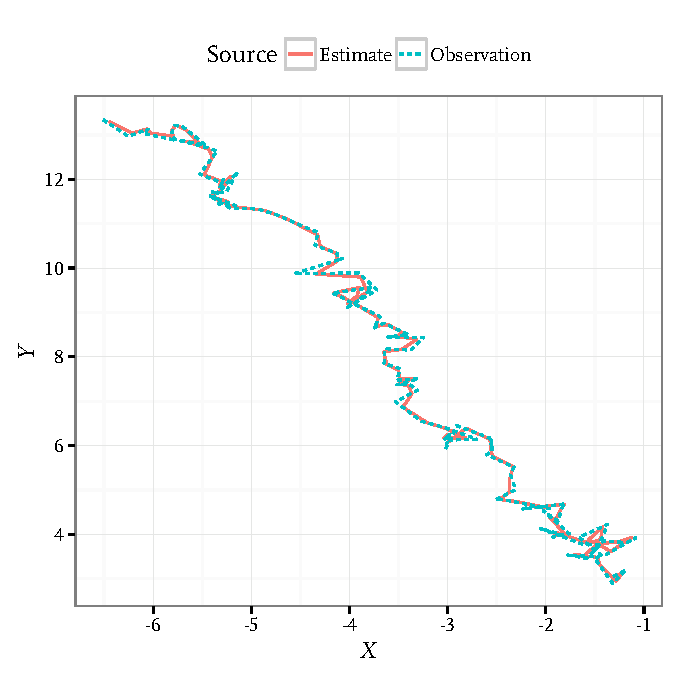
\includegraphics{fig/pf}
  \caption{Estimates and observations of the particle filter}
  \label{fig:pf}
\end{figure}

\chapter{Symmetric multiprocessing}
\label{chap:Symmetric multiprocessing}

Many Monte Carlo algorithms admit straight forward parallelism. In this
chapter, we introduce how to use the library to parallelize a Monte Carlo
algorithm implementations on shared memory symmetric multiprocessing (\smp)
platforms.

\section{Decomposition of evaluation objects}
\label{sec:Decomposition of evaluation objects}

Recall that, in section~\ref{sec:Sampler} we introduced the concepts of sampler
evaluation objects. The primary method of iterating a sampler is through
one or more evaluation objects that is convertible to the following type,
\begin{Verbatim}
  using eval_type = std::function<void(std::size_t, Particle<T> &)>;
\end{Verbatim}
In some situations, part of the evaluation process can be parallelized. For
example, consider the weight step in the simple particle filter in
section~\ref{sec:Example (Core concepts)}. Recall the simple \verb|PFWeight|
function in section~\ref{sub:Implementation (PF)},
\begin{Verbatim}
  inline void PFWeight(std::size_t iter, Particle<PF> &particle)
  {
      Vector<double> weight(particle.size());
      for (auto idx : particle)
          weight[idx.i()] = idx.log_likelihood(iter);
      particle.weight().add_log(weight.data());
  }
\end{Verbatim}
The loop inside the function can be parallelized, since the assignment is
independent of each other. However, the statements before and after the loop
cannot be parallelized. Therefore, we can decompose it into three simple
functions. Below, we re-implement \verb|PFWeight| as a class that is
convertible to \verb|eval_type|.
\begin{Verbatim}
  class PFWeight
  {
      public:
      void operator()(std::size_t iter, Particle<PF> &particle)
      {
          eval_first(iter, particle);
          for (auto idx : particle)
              eval_each(idx);
          eval_last(iter, particle);
      }

      void eval_first(std::size_t, Particle<PF> &particle)
      {
          weight_.resize(particle.size());
      }

      void eval_each(std::size_t iter, ParticleIndex<PF> idx)
      {
          weight_[idx.i()] = idx.log_likelihood(iter);
      }

      void eval_last(std::size_t, Particle<PF> &particle)
      {
          particle.weight().add_log(weight_.data());
      }

      private:
      Vector<double> weight_;
  }; // class PFWeight
\end{Verbatim}
Of course, such an implementation provides no benefits compared to the
original. In fact it is rather cumbersome. However, the library provides a
simple mechanism to convert any operators implemented this way to a
parallelized one. For example,
\begin{Verbatim}
  class PFWeightSMP : public SamplerEvalSMP<PF>
  {
      public:
      void eval_first(std::size_t, Particle<PF> &particle)
      {
          weight_.resize(particle.size());
      }

      void eval_each(std::size_t iter, ParticleIndex<PF> idx)
      {
          weight_[idx.i()] = idx.log_likelihood(iter);
      }

      void eval_last(std::size_t, Particle<PF> &particle)
      {
          particle.weight().add_log(weight_.data());
      }

      private:
      Vector<double> weight_;
  }; // class PFWeight
\end{Verbatim}
This new implementation differs from the one earlier in two places. First, it
is now a derived class of \verb|SamplerEvalSMP<PF>|. Second, the interface
operator, which makes the class type convertible to \verb|eval_type| of
\verb|Sampler| is removed. Now, the loop inside that operator in earlier
implementations will be parallelized. Still, for this simple function, the
performance benefits through parallelization is minimal. However, in less
trivial situations, \verb|eval_each| may be substantially more complicated. And
the extra effort to decompose the implementation into these three functions
will be minimal and there can be considerable performance advantage.

\subsection{The \texttt{SamplerEvalSMP} class}
\label{sub:The SamplerEvalSMP class}

We have already seen the \verb|SamplerEvalSMP| class template. The full
declaration of the template is as below,
\begin{Verbatim}
  template <typename T, typename = Virtual, typename = BackendSMP>
  class SamplerEvalSMP;
\end{Verbatim}
The first template parameter is the same as that of \verb|Sampler|. The second
specifies the polymorphism method. The default is to use virtual functions. We
will introduce another method later in section~\ref{sec:Static polymorphism}.
The last one selects the parallel programming models, or ``backends''. The
default is platform dependent and will be detailed in
section~\ref{sec:Programming models}. In this section, we will discuss the
default behavior.

The class template has one public method.
\begin{Verbatim}
  void operator()(std::size_t iter, Particle<T> &particle);
\end{Verbatim}
This makes instances of its derived classes convertible to \verb|eval_type| of
\verb|Sampler|. Its constructors and other special members are protected. And
thus it cannot be used on its own. It also has three other protected members,
\begin{Verbatim}
    virtual void eval_first(std::size_t, Particle<T> &);
    virtual void eval_each(std::size_t, ParticleIndex<T>);
    virtual void eval_last(std::size_t, Particle<T> &);
\end{Verbatim}
The default implementation of each is to do nothing. They are not pure virtual
functions, and thus their implementation in the derived class is optional. The
public operator is implemented as if it is the same as we saw earlier in the
\verb|PFWeight| class. How the loop is parallelized is implementation detail.
The only requirement is that the derived class implementation of
\verb|eval_each| has to be thread-safe.

A full treatment of thread-safety is beyond the scope of this manual. Here are
rule of thumbs. In the standard library, this library and others designed with
thread-safety in mind, one can usually assume the following,
\begin{itemize}
  \item Namespace scope functions are thread-safe.
  \item Constant member functions are thread-safe.
  \item Non-constant member functions are \emph{potentially not} thread-safe.
\end{itemize}
Note that, constant member function is often a sufficient, but not necessary
condition for thread-safety. For example, the \verb|eval_each| method itself is
a non-constant member function, but it is required to be thread-safe.

Here is one example of a problematic implementation of \verb|eval_each|,
\begin{Verbatim}
  using T = StateMatrix<RowMajor, 1, double>;

  class Eval : SamplerEvalSMP<T>
  {
      public:
      void eval_each(std::size_t iter, ParticleIndex<T> idx)
      {
          idx(0) = normal_(rng_);
      }

      private:
      std::mt19937 rng_;
      std::normal_distribution<double> normal_;
  };
\end{Verbatim}
The methods \verb|operator()| of \rng engines and the distribution generators
are generally non-constant members. And therefore they are potentially not
thread-safe. In fact, in the above example, they are indeed so. And when
parallelized the behavior is undefined. The correct way is to construct the
distribution object within \verb|eval_each| and use the \rng engines in the
particle system,
\begin{Verbatim}
  class Eval : SamplerEvalSMP<T>
  {
      public:
      void eval_each(std::size_t iter, ParticleIndex<T> idx)
      {
          std::normal_distribution<double> normal_;
          idx(0) = normal_(idx.rng());
      }
  };
\end{Verbatim}

\subsection{The \texttt{MonitorEvalSMP} class}
\label{sub:he MonitorEvalSMP class}

A function or class that is convertible to \verb|eval_type| of \verb|Monitor|
can also be parallelized. This is done through the following class template,
\begin{Verbatim}
  template <typename T, typename = Virtual, typename = BackendSMP>
  class MonitorEvalSMP;
\end{Verbatim}
This is similar to \verb|SamplerEvalSMP| except for the \verb|eval_each|
method, which has the following signature,
\begin{Verbatim}
  virtual void eval_each(
      std::size_t iter, std::size_t dim, ParticleIndex<T> idx, double *r);
\end{Verbatim}
Now the output parameter \verb|r| no longer points an $N$ by $d$ matrix.
Instead it points to a $d$-vector specific for each particle. For example,
recall the \verb|PFEstimate| function in section~\ref{sub:Implementation (PF)}.
\begin{Verbatim}
  inline void PFEstimate(
      std::size_t, std::size_t, Particle<PF> &particle, double *r)
  {
      for (auto idx : particle) {
          *r++ = idx.pos_x();
          *r++ = idx.pos_y();
      }
  }
\end{Verbatim}
This can be parallelized as the following,
\begin{Verbatim}
  class PFEstimate : public MonitorEvalSMP<PF>
  {
      public:
      void eval_each(
          std::size_t, std::size_t, ParticleIndex<PF> idx, double *r)
      {
          *r++ = idx.pos_x();
          *r++ = idx.pos_y();
      }
  }; // class PFEstimate
\end{Verbatim}
Optionally, the derived class can also have \verb|eval_first| and
\verb|eval_last| methods, similar to that of \verb|SamplerEvalSMP|.

\section{Static polymorphism}
\label{sec:Static polymorphism}

Calling virtual functions has a small cost at runtime. There are situations
where there is a large number of particles, and thus parallelization is
beneficial, but the computation of \verb|eval_each| is light weighted and the
cost of virtual function calls becomes significant. In this case, one can
specify the second template parameter of \verb|SamplerEvalSMP| and
\verb|MonitorEvalSMP| to force the compiler to statically dispatch calls of
\verb|eval_each|. For example,
\begin{Verbatim}
  class Eval : SamplerEvalSMP<T, Derived>;
\end{Verbatim}
The class \verb|Derived| is where the base class \emph{start} looking for
methods \verb|eval_each|, etc. It does not have to implement these methods
itself. For example,
\begin{Verbatim}
  template <typename Derived>
  class Eval : public SamplerEvalSMP<T, Derived>
  {
      public:
      void eval_first(std::size_t iter, Particle<T> &particle);
  };

  class Eval1 : public Eval<Eval1>
  {
      public:
      void eval_each(std::size_t iter, ParticleIndex<T> idx);
  };

  class Eval2 : public Eval<Eval2>
  {
      public:
      void eval_each(std::size_t iter, ParticleIndex<T> idx);
  };
\end{Verbatim}
Here, \verb|Eval| is a direct derived class of \verb|SamplerEvalSMP|, and it
implements the \verb|eval_first| method. This method is inherited by
\verb|Eval1| and \verb|Eval2|, which implement the \verb|eval_each| method. The
base class \verb|SamlerEvalSMP| will start looking for \verb|eval_first| in
\verb|Eval1| and \verb|Eval2|. But it will find it in \verb|Eval|. It will
find \verb|eval_each| in those two classes. And it will find \verb|eval_last|
in itself.\footnote{This is not actually true. It will find unimplemented
  methods in its base class. However this is an implementation detail.}

The implementations of methods \verb|eval_each| etc., can be either constant,
non-constant, or static. This type of use is call \emph{Curiously Recurring
  Template Pattern} (\crtp\footnote{%
  \url{https://en.wikipedia.org/wiki/Curiously_recurring_template_pattern}}).
The key point is that, the template parameter \verb|Derived| tells
\verb|SamlerEvalSMP| where should it start looking for \verb|eval_each|, etc.
And it will cast itself to \verb|Derived| if it finds non-static member
functions. It will call the methods directly if it finds static member
functions. The class template \verb|SamplerEvalSMP| has \emph{non-virtual}
default implementations of these methods.

\section{Programming models}
\label{sec:Programming models}

The third template parameter of \verb|SamplerEvalSMP| and \verb|MonitorEvalSMP|
specifies the programming model to use for parallelization. Possible types are
\begin{Verbatim}
  class BackendSEQ; // Sequential implementation
  class BackendSTD; // Parallelization using the standard library
  class BackendOMP; // Parallelization using OpenMP
  class BackendTBB; // Parallelization using Intel TBB
\end{Verbatim}
It is also possible to implement new backends by partial specialization of
\verb|SamplerEvalSMP| and \verb|MonitorEvalSMP|. However, this is a too
technical topic to be included in this manual.

Each partial specialization of \verb|SamplerEvalSMP| for the types above has a
protected method,
\begin{Verbatim}
  template <typename... Args>
  void run(std::size_t iter, Particle<T> &particle, std::size_t grainsize,
      Args &&... args);
\end{Verbatim}
which is called by the public operator method. One may use this function to
gain finer control of the parallelization. The behavior and allowable arguments
depend on the specific programming model. At the time of writing, this only has
effects on the \tbb backend. For others, these arguments are ignored.

In the case of \tbb, one can control the task division through the grain size.
For example,
\begin{Verbatim}
  class Eval : SamplerEvalSMP<T, Eval, BackendTBB>
  {
      public:
      void operator()(std::size_t iter, Particle<T> &particle)
      {
          run(iter, particle, G);
      }

      void eval_each(std::size_t, ParticleIndex<T> idx);
  };
\end{Verbatim}
The argument $G$ passed to \verb|run| above controls the threading such that,
each thread will process at least $G / 2$ particles. See the documents of \tbb
for more information of grain size. The additional arguments \verb|args| are
passed directly as the optional arguments of \verb|tbb::parallel_for|, the
partitioner and the task group context. See documents of \tbb for more details.

\section{Vectorization}
\label{sec:Vectorization}

It is often more efficient to process a vector as a whole instead of through a
loop. For example, considering the task of initializing states from a Gamma
distribution,
\begin{Verbatim}
  using T = StateMatrix<ColMajor, 1, double>;

  class Eval
  {
      public:
      void operator()(std::size_t iter, Particle<T> &particle)
      {
          std::gamma_distribution<double> gamma(2, 1);
          auto &rng = particle.rng();
          for (auto idx : particle)
              idx(0) = gamma(rng);
      }
  };
\end{Verbatim}
Later in section~\ref{sec:Vectorized random number generating} we will show
that the library provides vectorized random numbers generating. For example,
the above can be written as,
\begin{Verbatim}
  class Eval
  {
      public:
      void operator()(std::size_t iter, Particle<T> &particle)
      {
          GammaDistribution<double> gamma(2, 1);
          auto &rng = particle.rng();
          auto n = particle.size();
          auto r = particle.state().col_data(0);
          rand(rng, gamma, n, r);
      }
  };
\end{Verbatim}
which is about four to five times faster than the loop earlier. This is called
\emph{vectorization}. However, if the sample size is large, we would also like
to parallelize the loop. It is not possible to combine vectorization and
parallelization through the \verb|eval_each| method we have seen. In this
situation, instead of implementing \verb|eval_each|, one can implement an
\verb|eval_range| method. For example,
\begin{Verbatim}
  class Eval : public SamplerEvalSMP<T>
  {
      public:
      void eval_range(std::size_t iter, const ParticleRang<T> &range)
      {
          GammaDistribution<double> gamma(2, 1);
          auto &rng = range.begin().rng();
          auto n = range.size();
          auto r = range.particle().state().col_data(0) + range.first();
          rand(rng, gamma, n, r);
      }
  };
\end{Verbatim}
The class \verb|ParticleRange| is an abstraction of a subset of a particle
system. It has the following methods,
\begin{Verbatim}
  range.particle();     // A reference to the particle system it belongs to
  range.particle_ptr(); // A pointer to the particle system it belongs to
  range.first(); // The index of the first particle within the range
  range.last();  // The index of one pass the last particle within the range
  range.begin(); // An ParticleIndex<T> object for the first particle
  range.end();   // An ParticleIndex<T> object for one pass the last particle
\end{Verbatim}
It can also be iterated, similar to \verb|Particle|. For example,
\begin{Verbatim}
  for (auto idx : range)
      /* process ParticleIndex<T> object idx */;
\end{Verbatim}
If such a method is defined, the particle system will first be partitioned into
multiple disjoint ranges. And each thread will process one of more of such
ranges. The \verb|eval_range| method has to be thread-safe. If both
\verb|eval_range| and \verb|eval_each| are defined, the later is ignored.

\subsection{Using \texttt{eval\_range} with \tbb}

When using the \tbb backend, special care need to be taken when using the
\verb|eval_range| implementation. The purpose of using \verb|eval_range|
instead of \verb|eval_each| is to process vectors as a whole. For optimal
performance, the vectors cannot be too short. Otherwise, the performance will
only be worse than using a loop. Therefore it is important to control the grain
size. Therefore, it is recommended that if one does want to use
\verb|eval_range|, then one should also redefine the interface operator. For
example,
\begin{Verbatim}
  class Eval : public SamplerEvalSMP<T>
  {
      public:
      void operator()(std::size_t iter, Particle<T> &particle)
      {
          run(iter, particle, G);
      }

      void eval_range(std::size_t iter, const ParticleRang<T> &range);
  };
\end{Verbatim}
where $G$ is the grain size. Even though the grain size has no effect for
backends other than \tbb at the moment, it is planned to provide similar
functionality as \tbb for other backends in the near future.

% ============================================================================
%  MCKL/manual/tex/resample.tex
% ----------------------------------------------------------------------------
%  MCKL: Monte Carlo Kernel Library
% ----------------------------------------------------------------------------
%  Copyright (c) 2013-2016, Yan Zhou
%  All rights reserved.
%
%  Redistribution and use in source and binary forms, with or without
%  modification, are permitted provided that the following conditions are met:
%
%    Redistributions of source code must retain the above copyright notice,
%    this list of conditions and the following disclaimer.
%
%    Redistributions in binary form must reproduce the above copyright notice,
%    this list of conditions and the following disclaimer in the documentation
%    and/or other materials provided with the distribution.
%
%  THIS SOFTWARE IS PROVIDED BY THE COPYRIGHT HOLDERS AND CONTRIBUTORS "AS IS"
%  AND ANY EXPRESS OR IMPLIED WARRANTIES, INCLUDING, BUT NOT LIMITED TO, THE
%  IMPLIED WARRANTIES OF MERCHANTABILITY AND FITNESS FOR A PARTICULAR PURPOSE
%  ARE DISCLAIMED. IN NO EVENT SHALL THE COPYRIGHT HOLDER OR CONTRIBUTORS BE
%  LIABLE FOR ANY DIRECT, INDIRECT, INCIDENTAL, SPECIAL, EXEMPLARY, OR
%  CONSEQUENTIAL DAMAGES (INCLUDING, BUT NOT LIMITED TO, PROCUREMENT OF
%  SUBSTITUTE GOODS OR SERVICES; LOSS OF USE, DATA, OR PROFITS; OR BUSINESS
%  INTERRUPTION) HOWEVER CAUSED AND ON ANY THEORY OF LIABILITY, WHETHER IN
%  CONTRACT, STRICT LIABILITY, OR TORT (INCLUDING NEGLIGENCE OR OTHERWISE)
%  ARISING IN ANY WAY OUT OF THE USE OF THIS SOFTWARE, EVEN IF ADVISED OF THE
%  POSSIBILITY OF SUCH DAMAGE.
% ============================================================================

\chapter{Resampling}
\label{chap:Resampling}

Given a particle system $S_{1:N}$, $S_i = (X_i,W_i)$, a resampling algorithm
generate a new system $\hat{S}_{1:M}$ such that,
\begin{equation*}
  \Exp\Square[Big]{\sum_{i=1}^M{\hat{W}_i\varphi(\hat{X}_i)}} =
  \Exp\Square[Big]{\sum_{i=1}^N{W_i\varphi(X_i)}}
\end{equation*}
for test function $\varphi$. Regardless of other statistical properties, in
practice, such an algorithm can be decomposed into three steps,
\begin{enumerate}
  \item Generate an $N$-vector of replication numbers $r_{1:N}$, such that
    $\sum_{i=1}^N r_i = M$, and $0 \le r_i \le M$ for $i=1,\dots,N$.
  \item Generate an $M$-vector of indices $a_{1:M}$ such that $\sum_{j=1}^M
    \bbI_{\{i\}}(a_j) = r_i$, and $1 \le a_i \le N$ for $i = 1,\dots,M$.
  \item Set $\hat{X}_i = X_{a_i}$ for $i = 1,\dots,M$.
\end{enumerate}
Given the results of the first step, the second step can be implemented with a
deterministic algorithm. And the final results will be determined up to
re-ordering. Therefore, it is the first step that determines the statistical
properties of the new particle system.

\section{Using resampling with sampler}
\label{sec:Using resampling with sampler}

Recall Section~\ref{sec:Sampler}, any object that is convertible to,
\begin{Verbatim}
  using eval_type =
      std::function<void(size_t, Particle<T> &)>;
\end{Verbatim}
can be added as a resampling evaluation object to a \verb|Sampler| object. The
library defines the following class template,
\begin{Verbatim}
  template <typename T>
  class ResampleEval;
\end{Verbatim}
that is compatible with the type above. It has a single constructor,
\begin{Verbatim}
  explicit ResampleEval(const eval_type &eval);
\end{Verbatim}
where \verb|eval_type| (not to be confused with the type of the same name in
\verb|Sampler|) is defined as the following,
\begin{Verbatim}
  using eval_type = std::function<void(
          size_t,
          size_t,
          typename Particle<T>::rng_type &,
          const double *,
          typename Particle<T>::size_type *)>;
\end{Verbatim}
An evaluation object that is convertible to the above will be used to generate
the $N$-vector of replication numbers $r_{1:N}$. When called, it will be passed
the following arguments,
\begin{Verbatim}
  eval(N, M, rng, w, r);
\end{Verbatim}
where $N$ is the original sample size, $M$ is the new sample size, \verb|rng|
is an \rng engine, \verb|w| is a pointer to the $N$-vector of normalized
weights, and output parameter \verb|r| points to the $N$-vector of replication
numbers. One can define function templates to avoid declaring these parameter
types explicitly. An object of the class \verb|ResampleEval| is convertible to
\verb|eval_type| of \verb|Sampler|, and can be added to a sampler as a
resampling evaluation object. Its operator will call the object passed to its
constructor to generate the $N$-vector of replication numbers $r_{1:N}$. And it
will generate the the $M$-vector of indices $a_{1:M}$. And last, it will used
the \verb|select| method of type \verb|T| to duplicate states. The vector of
indices generated by this operator has the following property, in addition to
those stated earlier at the beginning of this chapter,
\begin{equation*}
  a_i = i \quad \text{if} \quad  r_i > 0 \quad
  \text{for } i = 1,\dots,\min\{N, M\}
\end{equation*}
In fact, the \verb|select| method of \verb|StateMatrix| in
Section~\ref{sec:State} makes the assumptions of this property about its input
indices.

\section{Algorithm}
\label{sec:Algorithm}

The library implements all algorithms discussed in \textcite{Douc:2005wa} and
two extensions to the those algorithms. Samplers can be constructed with
builtin algorithms as seen in Section~\ref{sec:Sampler}. All builtin algorithms
are implemented in the following class template,
\begin{Verbatim}
  template <typename U01SeqType, bool Residual>
  class ResampleAlgorithm;
\end{Verbatim}
We will explain the template parameters later. This class has the following
interface,
\begin{Verbatim}
  template <
      typename RNGType,
      typename InputIter,
      typename OutputIter>
  void eval(
      size_t N,
      size_t M,
      RNGType &rng,
      InputIter w,
      OutputIter r) const
\end{Verbatim}
Its parameters are as those described earlier for \verb|eval_type| of
\verb|ResampleEval|. The algorithm that it implements depends on the template
parameters of the class. The type \verb|U01SeqType| shall be a class type with
a default constructor and a call operator. It shall be able to be used as the
following,
\begin{Verbatim}
  typename std::iterator_traits<IntputIter>::value_type *u;
  // allocate space for u
  U01SeqType u01seq;
  u01seq(rng, R, u);
\end{Verbatim}
After the call, it shall generate a sequence $0 \le U_1 \le \dots\le U_R < 1$.
The library provides three implementations, which will be discussed in the next
section. The algorithm proceeds as the following to generate $r_{1:N}$,
\begin{algorithmic}
  \REQUIRE $\sum_{i=1}^N W_i = 1$
  \IF{\texttt{Residual} is false}
  \STATE $r_i \leftarrow 0$ for $i = 1,\dots,N$
  \STATE $R \leftarrow M$
  \ELSE
  \STATE $r_i \leftarrow \Floor{MW_i}$ for $i = 1,\dots,N$
  \STATE $R \leftarrow M - \sum_{i=1}^N r_i$
  \STATE $W_i \leftarrow MW_i - r_i$ for $i = 1,\dots,N$
  \STATE $W_i \leftarrow W_i / \sum_{i=1}^NW_i$
  \ENDIF
  \STATE Generate $U_{1:R}$ using \verb|U01SeqType|
  \STATE $V_0 \leftarrow 0$, $V_i \leftarrow V_{i - 1} + W_i$ for $i =
  1,\dots,N$.
  \STATE $r_i \leftarrow r_i + \sum_{j=1}^R\bbI_{[V_{i-1},V_i)}(U_j)$
\end{algorithmic}
All builtin schemes differ only in their choices of the template parameters
\verb|U01SeqType| and \verb|Residual|. There are three implementations in the
library of the uniform sequence,

\subsubsection{Sorted sequence}

The class,
\begin{Verbatim}
  class U01SequenceSorted;
\end{Verbatim}
generates the sequence $U_{1:R}$ such that it has the same distribution as a
sorted sequence of i.i.d.\ standard uniform random variables $V_{1:R}$.

\subsubsection{Stratified sequence}

The class
\begin{Verbatim}
  class U01SequenceStratified;
\end{Verbatim}
generates the sequence $U_{1:R}$ such that $U_i = (i - 1)\delta + V_i\delta$
where $V_{1:R}$ are i.i.d.\ standard uniform random variables.

\subsubsection{Systematic sequence}

The class
\begin{Verbatim}
  class U01SequenceSystematic;
\end{Verbatim}
generates the sequence $U_{1:R}$ such that $U_i = (i - 1)\delta + V\delta$
where $V$ is a standard uniform random variable.

All the builtin algorithms are listed in Table~\ref{tab:Resampling schemes}.
Convenient type aliases are also defined,
\begin{Verbatim}
  using ResampleMultinomial =
      ResampleAlgorithm<U01SequenceSorted, false>;

  using ResampleStratified =
      ResampleAlgorithm<U01SequenceStratified, false>;

  using ResampleSystematic =
      ResampleAlgorithm<U01SequenceSystematic, false>;

  using ResampleResidual =
      ResampleAlgorithm<U01SequenceSorted, true>;

  using ResampleResidualStratified =
      ResampleAlgorithm<U01SequenceStratified, true>;

  using ResampleResidualSystematic =
      ResampleAlgorithm<U01SequenceSystematic, true>;
\end{Verbatim}

\begin{table}
  \begin{tabularx}{\textwidth}{lLl}
    \toprule
    \verb|ResampleScheme| & \verb|U01SeqType| & \verb|Residual| \\
    \midrule
    \verb|Multinomial|        & \verb|U01SequenceSorted|     & \verb|false| \\
    \verb|Stratified|         & \verb|U01SequenceStratified| & \verb|false| \\
    \verb|Systematic|         & \verb|U01SequenceSystematic| & \verb|false| \\
    \verb|Residual|           & \verb|U01SequenceSorted|     & \verb|true|  \\
    \verb|ResidualStratified| & \verb|U01SequenceStratified| & \verb|true|  \\
    \verb|ResidualSystematic| & \verb|U01SequenceSystematic| & \verb|true|  \\
    \bottomrule
  \end{tabularx}
  \caption{Resampling schemes}
  \label{tab:Resampling schemes}
\end{table}

% ============================================================================
%  MCKL/manual/tex/math.tex
% ----------------------------------------------------------------------------
%  MCKL: Monte Carlo Kernel Library
% ----------------------------------------------------------------------------
%  Copyright (c) 2013-2016, Yan Zhou
%  All rights reserved.
%
%  Redistribution and use in source and binary forms, with or without
%  modification, are permitted provided that the following conditions are met:
%
%    Redistributions of source code must retain the above copyright notice,
%    this list of conditions and the following disclaimer.
%
%    Redistributions in binary form must reproduce the above copyright notice,
%    this list of conditions and the following disclaimer in the documentation
%    and/or other materials provided with the distribution.
%
%  THIS SOFTWARE IS PROVIDED BY THE COPYRIGHT HOLDERS AND CONTRIBUTORS "AS IS"
%  AND ANY EXPRESS OR IMPLIED WARRANTIES, INCLUDING, BUT NOT LIMITED TO, THE
%  IMPLIED WARRANTIES OF MERCHANTABILITY AND FITNESS FOR A PARTICULAR PURPOSE
%  ARE DISCLAIMED. IN NO EVENT SHALL THE COPYRIGHT HOLDER OR CONTRIBUTORS BE
%  LIABLE FOR ANY DIRECT, INDIRECT, INCIDENTAL, SPECIAL, EXEMPLARY, OR
%  CONSEQUENTIAL DAMAGES (INCLUDING, BUT NOT LIMITED TO, PROCUREMENT OF
%  SUBSTITUTE GOODS OR SERVICES; LOSS OF USE, DATA, OR PROFITS; OR BUSINESS
%  INTERRUPTION) HOWEVER CAUSED AND ON ANY THEORY OF LIABILITY, WHETHER IN
%  CONTRACT, STRICT LIABILITY, OR TORT (INCLUDING NEGLIGENCE OR OTHERWISE)
%  ARISING IN ANY WAY OUT OF THE USE OF THIS SOFTWARE, EVEN IF ADVISED OF THE
%  POSSIBILITY OF SUCH DAMAGE.
% ============================================================================

\chapter{Elementary mathematical functions}
\label{chap:Elementary mathemtical functions}

\section{Constants}
\label{sec:Constants}

The library defines some mathematical constants in the form of constant
expression functions. For example, to get the value of $\pi$ with a desired
precision, one can use the following,
\begin{Verbatim}
  constexpr float pi_f = const_pi<float>();
  constexpr double pi_d = const_pi<double>();
  constexpr long double pi_l = const_pi<long double>();
\end{Verbatim}
The compiler will evaluate these values at compile-time and thus there is no
performance difference from hard-coding the constants in the program, while the
readability is improved. All defined constants are listed in
Table~\ref{tab:Mathematical constants}.

\section{Vectorized functions}
\label{sec:Vectorized functions}

The library provides a set of vectorized elementary mathematical functions.
For example, to perform additions of two vectors,
\begin{Verbatim}
  std::size_t n = 1000;
  Vector<double> a(n), b(n), y(n);
  // Fill vectors a and b
  add(n, a.data(), b.data(), y.data());
\end{Verbatim}
This is equivalent to,
\begin{Verbatim}
  for (std::size_t i = 0; i != n; ++i)
      y[i] = a[i] + b[i];
\end{Verbatim}
The functions defined are listed in Tables~\ref{tab:Arithmetic functions}
to~\ref{tab:Rounding functions}. For each function, the first parameter is
always the length of the vector, and the last is a pointer to the output vector
(except for \verb|sincos| and \verb|modf|, which have two output parameters).
For all functions, the output is always a vector. If there are more than one
input parameters, then some of them, but not all, can be scalars. For example,
for the function call \verb|fma(n, a, b, c, y)| in Table~\ref{tab:Arithmetic
  functions}, the input parameters are \verb|a|, \verb|b|, and \verb|c|. Some
of them, not all, can be scalars instead of pointers to vectors. The output
parameter \verb|y| has to be a pointer to a vector. Therefore, there are seven
versions of this function for each type of the value. Note that, mixed
precision is not allowed. For example,
\begin{Verbatim}
  Vector<double> a(n);
  Vector<double> b(n);
  Vector<double> y(n);
  fma(n, a.data(), b.data(), 2, y.data());
\end{Verbatim}
will cause compile-time error because the fourth argument \verb|2| is of type
\verb|int| while the others are of \verb|double| precision. The correct call
shall be,
\begin{Verbatim}
  fma(n, a.data(), b.data(), 2.0, y.data());
\end{Verbatim}
Without any third-party libraries, these functions do not provide performance
gain compared to the simple loop. When \mkl is present, some functions can have
substantial performance improvement when all input arguments are vectors. The
performance of vectorized random number generating introduced later in
Section~\ref{sec:Vectorized random number generating} heavily depends on these
functions.

\begin{table}
  \begin{tabularx}{\textwidth}{p{1.5in}Lp{1.5in}L}
    \toprule
    Function & Value & Function & Value \\
    \midrule
    \verb|const_inf|          & $\infty$        &
    \verb|const_nan|          & NaN             \\
    \verb|const_zero|         & $0$             &
    \verb|const_one|          & $1$             \\
    \verb|const_pi|           & $\pi$           &
    \verb|const_pi_2|         & $2\pi$          \\
    \verb|const_pi_inv|       & $1/\pi$         &
    \verb|const_pi_sqr|       & $\pi^2$         \\
    \verb|const_pi_by2|       & $\pi/2$         &
    \verb|const_pi_by3|       & $\pi/3$         \\
    \verb|const_pi_by4|       & $\pi/4$         &
    \verb|const_pi_by6|       & $\pi/6$         \\
    \verb|const_pi_2by3|      & $2\pi/3$        &
    \verb|const_pi_3by4|      & $3\pi/4$        \\
    \verb|const_pi_4by3|      & $4\pi/3$        &
    \verb|const_sqrt_pi|      & $\sqrt{\pi}$    \\
    \verb|const_sqrt_pi_2|    & $\sqrt{2\pi}$   &
    \verb|const_sqrt_pi_inv|  & $\sqrt{1/\pi}$  \\
    \verb|const_sqrt_pi_by2|  & $\sqrt{\pi/2}$  &
    \verb|const_sqrt_pi_by3|  & $\sqrt{\pi/3}$  \\
    \verb|const_sqrt_pi_by4|  & $\sqrt{\pi/4}$  &
    \verb|const_sqrt_pi_by6|  & $\sqrt{\pi/6}$  \\
    \verb|const_sqrt_pi_2by3| & $\sqrt{2\pi/3}$ &
    \verb|const_sqrt_pi_3by4| & $\sqrt{3\pi/4}$ \\
    \verb|const_sqrt_pi_4by3| & $\sqrt{4\pi/3}$ &
    \verb|const_ln_pi|        & $\ln{\pi}$      \\
    \verb|const_ln_pi_2|      & $\ln{2\pi}$     &
    \verb|const_ln_pi_inv|    & $\ln{1/\pi}$    \\
    \verb|const_ln_pi_by2|    & $\ln{\pi/2}$    &
    \verb|const_ln_pi_by3|    & $\ln{\pi/3}$    \\
    \verb|const_ln_pi_by4|    & $\ln{\pi/4}$    &
    \verb|const_ln_pi_by6|    & $\ln{\pi/6}$    \\
    \verb|const_ln_pi_2by3|   & $\ln{2\pi/3}$   &
    \verb|const_ln_pi_3by4|   & $\ln{3\pi/4}$   \\
    \verb|const_ln_pi_4by3|   & $\ln{4\pi/3}$   &
    \verb|const_e|            & $\EE$           \\
    \verb|const_e_inv|        & $1/\EE$         &
    \verb|const_sqrt_e|       & $\sqrt{\EE}$    \\
    \verb|const_sqrt_e_inv|   & $\sqrt{1/\EE}$  &
    \verb|const_sqrt_2|       & $\sqrt{2}$      \\
    \verb|const_sqrt_3|       & $\sqrt{3}$      &
    \verb|const_sqrt_5|       & $\sqrt{5}$      \\
    \verb|const_sqrt_10|      & $\sqrt{10}$     &
    \verb|const_sqrt_1by2|    & $\sqrt{1/2}$    \\
    \verb|const_sqrt_1by3|    & $\sqrt{1/3}$    &
    \verb|const_sqrt_1by5|    & $\sqrt{1/5}$    \\
    \verb|const_sqrt_1by10|   & $\sqrt{1/10}$   &
    \verb|const_ln_2|         & $\ln{2}$        \\
    \verb|const_ln_3|         & $\ln{3}$        &
    \verb|const_ln_5|         & $\ln{5}$        \\
    \verb|const_ln_10|        & $\ln{10}$       &
    \verb|const_ln_inv_2|     & $1/\ln{2}$      \\
    \verb|const_ln_inv_3|     & $1/\ln{3}$      &
    \verb|const_ln_inv_5|     & $1/\ln{5}$      \\
    \verb|const_ln_inv_10|    & $1/\ln{10}$     &
    \verb|const_ln_ln_2|      & $\ln\ln{2}$     \\
    \bottomrule
  \end{tabularx}
  \caption{Mathematical constants}
  \label{tab:Mathematical constants}
\end{table}

\begin{table}
  \begin{tabularx}{\textwidth}{LL}
    \toprule
    Function & Operation \\
    \midrule
    \verb|add(n, a, b, y)|    & $y_i = a_i + b_i$     \\
    \verb|sub(n, a, b, y)|    & $y_i = a_i - b_i$     \\
    \verb|sqr(n, a, y)|       & $y_i = a_i^2$         \\
    \verb|mul(n, a, b, y)|    & $y_i = a_i b_i$       \\
    \verb|abs(n, a, y)|       & $y_i = |a_i|$         \\
    \verb|fma(n, a, b, c, y)| & $y_i = a_i b_i + c_i$ \\
    \bottomrule
  \end{tabularx}
  \caption{Arithmetic functions}
  \label{tab:Arithmetic functions}
\end{table}

\begin{table}
  \begin{tabularx}{\textwidth}{LL}
    \toprule
    Function & Operation \\
    \midrule
    \verb|inv(n, a, y)|      & $y_i = 1 / a_i$              \\
    \verb|div(n, a, b, y)|   & $y_i = a_i / b_i$            \\
    \verb|sqrt(n, a, y)|     & $y_i = \sqrt{a_i}$           \\
    \verb|invsqrt(n, a, y)|  & $y_i = 1 / \sqrt{a_i}$       \\
    \verb|cbrt(n, a, y)|     & $y_i = \sqrt[3]{a_i}$        \\
    \verb|invcbrt(n, a, y)|  & $y_i = 1 / \sqrt[3]{a_i}$    \\
    \verb|pow2o3(n, a, y)|   & $y_i = a_i^{2/3}$            \\
    \verb|pow3o2(n, a, y)|   & $y_i = a_i^{3/2}$            \\
    \verb|pow(n, a, b, y)|   & $y_i = a_i^{b_i}$            \\
    \verb|hypot(n, a, b, y)| & $y_i = \sqrt{a_i^2 + b_i^2}$ \\
    \bottomrule
  \end{tabularx}
  \caption{Power and root functions}
  \label{tab:Power and root functions}
\end{table}

\begin{table}
  \begin{tabularx}{\textwidth}{LL}
    \toprule
    Function & Operation \\
    \midrule
    \verb|exp(n, a, y)|   & $y_i = \EE^{a_i}$     \\
    \verb|exp2(n, a, y)|  & $y_i = 2^{a_i}$       \\
    \verb|exp10(n, a, y)| & $y_i = 10^{a_i}$      \\
    \verb|expm1(n, a, y)| & $y_i = \EE^{a_i} - 1$ \\
    \verb|log(n, a, y)|   & $y_i = \ln a_i$       \\
    \verb|log2(n, a, y)|  & $y_i = \log_2 a_i$    \\
    \verb|log10(n, a, y)| & $y_i = \log_{10} a_i$ \\
    \verb|log1p(n, a, y)| & $y_i = \ln(a_i + 1)$  \\
    \bottomrule
  \end{tabularx}
  \caption{Exponential and logarithm functions}
  \label{tab:Exponential and logarithm functions}
\end{table}

\begin{table}
  \begin{tabularx}{\textwidth}{LL}
    \toprule
    Function & Operation \\
    \midrule
    \verb|cos(n, a, y)|       & $y_i = \cos(a_i)$                    \\
    \verb|sin(n, a, y)|       & $y_i = \sin(a_i)$                    \\
    \verb|sincos(n, a, y, z)| & $y_i = \sin(a_i)$, $z_i = \cos(a_i)$ \\
    \verb|tan(n, a, y)|       & $y_i = \tan(a_i)$                    \\
    \verb|acos(n, a, y)|      & $y_i = \arccos(a_i)$                 \\
    \verb|asin(n, a, y)|      & $y_i = \arcsin(a_i)$                 \\
    \verb|atan(n, a, y)|      & $y_i = \arctan(a_i)$                 \\
    \verb|acos(n, a, y)|      & $y_i = \arccos(a_i)$                 \\
    \verb|atan2(n, a, y)|     & $y_i = \arctan(a_i / b_i)$           \\
    \bottomrule
  \end{tabularx}
  \caption{Trigonometric functions}
  \label{tab:Trigonometric functions}
\end{table}

\begin{table}
  \begin{tabularx}{\textwidth}{LL}
    \toprule
    Function & Operation \\
    \midrule
    \verb|cosh(n, a, y)|  & $y_i = \cosh(a_i)$             \\
    \verb|sinh(n, a, y)|  & $y_i = \sinh(a_i)$             \\
    \verb|tanh(n, a, y)|  & $y_i = \tanh(a_i)$             \\
    \verb|acosh(n, a, y)| & $y_i = \mathrm{arc}\cosh(a_i)$ \\
    \verb|asinh(n, a, y)| & $y_i = \mathrm{arc}\sinh(a_i)$ \\
    \verb|atanh(n, a, y)| & $y_i = \mathrm{arc}\tanh(a_i)$ \\
    \bottomrule
  \end{tabularx}
  \caption{Hyperbolic functions}
  \label{tab:Hyperbolic functions}
\end{table}

\begin{table}
  \begin{tabularx}{\textwidth}{LL}
    \toprule
    Function & Operation \\
    \midrule
    \verb|erf(n, a, y)|     & $y_i = \mathrm{erf}(a_i)$                     \\
    \verb|erfc(n, a, y)|    & $y_i = \mathrm{erfc}(a_i)$                    \\
    \verb|cdfnorm(n, a, y)| & $y_i = 1 - \mathrm{erfc}(a_i / \sqrt{2}) / 2$ \\
    \verb|lgamma(n, a, y)|  & $y_i = \ln\Gamma(a_i)$                        \\
    \verb|tgamma(n, a, y)|  & $y_i = \Gamma(a_i)$                           \\
    \bottomrule
  \end{tabularx}
  \caption{Special functions}
  \label{tab:Special functions}
\end{table}

\begin{table}
  \begin{tabularx}{\textwidth}{LL}
    \toprule
    Function & Operation \\
    \midrule
    \verb|floor(n, a, y)| & $y_i = \Floor{a_i}$                        \\
    \verb|ceil(n, a, y)|  & $y_i = \Ceil{a_i}$                         \\
    \verb|trunc(n, a, y)| & $y_i = \mathrm{sgn}(a_i)\Floor{\Abs{a_i}}$ \\
    \verb|round(n, a, y)| & $y_i = \text{ nearest integer of }a_i$     \\
    \verb|modf(n, a, y, z)| &
    $y_i = \mathrm{sign}(a_i)\Floor{\Abs{a_i}}$,
    $z_i = \mathrm{sign}(a_i)\Abs{a_i - y_i}$ \\
    \bottomrule
  \end{tabularx}
  \caption{Rounding functions}
  \label{tab:Rounding functions}
\end{table}

\clearpage

% ============================================================================
%  MCKL/manual/tex/random.tex
% ----------------------------------------------------------------------------
%  MCKL: Monte Carlo Kernel Library
% ----------------------------------------------------------------------------
%  Copyright (c) 2013-2016, Yan Zhou
%  All rights reserved.
%
%  Redistribution and use in source and binary forms, with or without
%  modification, are permitted provided that the following conditions are met:
%
%    Redistributions of source code must retain the above copyright notice,
%    this list of conditions and the following disclaimer.
%
%    Redistributions in binary form must reproduce the above copyright notice,
%    this list of conditions and the following disclaimer in the documentation
%    and/or other materials provided with the distribution.
%
%  THIS SOFTWARE IS PROVIDED BY THE COPYRIGHT HOLDERS AND CONTRIBUTORS "AS IS"
%  AND ANY EXPRESS OR IMPLIED WARRANTIES, INCLUDING, BUT NOT LIMITED TO, THE
%  IMPLIED WARRANTIES OF MERCHANTABILITY AND FITNESS FOR A PARTICULAR PURPOSE
%  ARE DISCLAIMED. IN NO EVENT SHALL THE COPYRIGHT HOLDER OR CONTRIBUTORS BE
%  LIABLE FOR ANY DIRECT, INDIRECT, INCIDENTAL, SPECIAL, EXEMPLARY, OR
%  CONSEQUENTIAL DAMAGES (INCLUDING, BUT NOT LIMITED TO, PROCUREMENT OF
%  SUBSTITUTE GOODS OR SERVICES; LOSS OF USE, DATA, OR PROFITS; OR BUSINESS
%  INTERRUPTION) HOWEVER CAUSED AND ON ANY THEORY OF LIABILITY, WHETHER IN
%  CONTRACT, STRICT LIABILITY, OR TORT (INCLUDING NEGLIGENCE OR OTHERWISE)
%  ARISING IN ANY WAY OUT OF THE USE OF THIS SOFTWARE, EVEN IF ADVISED OF THE
%  POSSIBILITY OF SUCH DAMAGE.
% ============================================================================

\chapter{Random number generating}
\label{chap:Random number generating}

The library has a comprehensive \rng system to facilitate implementation of
Monte Carlo algorithms. Similar to the standard library header \verb|<random>|,
there are mainly two parts of this system. The first is a set of \rng{} engines
that generate random integers. The other is a set of distribution generators.
The former are documented in Sections~\ref{sec:Counter-based RNG}
to~\ref{sec:MKL RNG}, and the later in Section~\ref{sec:Distributions}. Apart
from these, the library also provides facilities for vectorized random number
generating (Section~\ref{sec:Vectorized random number generating}) and using
multiple \rng{}s in parallel programs (Section~\ref{sec:Multiple RNG streams}).
There are also some performance data in Appendix~\appref{chap:Performance of
  random number generators} and~\appref{chap:Performance of distribution
  generators}.

\section{Vectorized random number generating}
\label{sec:Vectorized random number generating}

Before we discuss other features, we first introduce a generic function
\verb|rand|, which provides vectorized random number generating. There are two
versions. The first operates on \rng engines and generates random integers,
\begin{Verbatim}
  template <typename RNGType>
  inline void rand(
      RNGType &rng,
      std::size_t n,
      typename RNGType::result_type *r);
\end{Verbatim}
The effect of the function call,
\begin{Verbatim}
  rand(rng, n, r);
\end{Verbatim}
is equivalent to the loop,
\begin{Verbatim}
  for (std::size_t i = 0; i != n; ++i)
      r[i] = rng();
\end{Verbatim}
The results will always be the same unless a non-deterministic \rng is used.
For some \rng{}s implemented in the library, the vectorized version may have
considerable performance advantage.

The second version of \verb|rand| is for generating distribution random
numbers,
\begin{Verbatim}
  template <typename RNGType, typename DistributionType>
  inline void rand(
      RNGType &rng,
      const DistributionType &distribution,
      std::size_t n,
      typename DistributionType::result_type *r);
\end{Verbatim}
For example,
\begin{Verbatim}
  NormalDistribution<double> normal;
  rand(rng, normal, n, r);
\end{Verbatim}
This is similar to the following loop,
\begin{Verbatim}
  for (std::size_t i = 0; i != n; ++i)
      r[i] = normal(rng);
\end{Verbatim}
Depending on the type of \verb|rng| and the distribution (including its
parameters), the vectorized version may have superior performance. However, the
results will not be exactly the same as using a loop.

For consistency, the library also defines the function \verb|rand| for
generating only one random number,
\begin{Verbatim}
  rand(rng);               // rng();
  rand(rng, distribution); // distribution(rng);
\end{Verbatim}
And each \rng engine and distribution generator also has methods for vectorized
generating,
\begin{Verbatim}
  rng(n, r);               // rand(rng, n, r);
  distribution(rng, n, r); // rand(rng, distribution, n, r);
\end{Verbatim}
To write generic functions, it is recommended to use the function \verb|rand|
instead of the member methods, since the former also works with classes not
defined by this library, such as those in the standard library.

\section{Counter-based \protect\rng}
\label{sec:Counter-based RNG}

The standard library provides a set of \rng engines. Unfortunately, none of
them are suitable for parallel computing without considerable efforts. To
illustrate the problem, consider the situation where there are two threads that
need to generate random numbers. And thus two \rng engine instances need to be
created for each thread. Let the random numbers generated by them be
$\{r_i^1\}_{i>0}$ and $\{r_i^2\}_{i>0}$. Because of the deterministic and
recursive natural of the these \rng{}s, there exists $k\in\Integer$, such that,
$r_i^1 = r_{i + k}^2$ for all $i > \max\{0, -k\}$. If $\Abs{k}$ is larger than
or close to the total number of random numbers required in each thread, then
this situation might not be an issue. However, there is no easy way to ensure
such a condition.

There are two standard solutions to this problem. The first is to use
sub-streams for each thread. For example,
\begin{Verbatim}
  std::mt19937 rng;

  // Thread k
  std::mt19937 rng_k = rng;
  rng_k.discard(n * k);
\end{Verbatim}
where $n$ is the number of random numbers required by each thread. The $k$\ith
thread only uses the random numbers in the sub-stream $\{r_i\}_{nk < i \le
  n(k+1)}$. For this to work, the \rng needs a fast \verb|discard|
implementation, preferably with $\calO(1)$ cost. In addition, one needs to
manage \rng{}s explicitly for each thread, which prevents this method to be
used in environments where threads are created implicitly, such as using \tbb
for parallelization.

The second solution is to use a leap-frog algorithm, such that each thread will
use the elements $\{r_{iK + k}\}_{i>0}$ of the stream, where $K$ is the total
number of threads. This is not directly supported in the standard library, but
can be emulated,
\begin{Verbatim}
  std::mt19937 rng;

  // Thread k
  std::mt19937 tmp = rng;
  tmp.discard(k);
  std::discard_block_engine<std::mt19937, K, 1> rng_k(tmp);
\end{Verbatim}
This not only requires managing the \rng{}s explicitly, but also knowing the
number of threads at compile-time, which prevents it to be used in any
applications using dynamic parallelization. And similar to the first solution,
it cannot be used when threads are created implicitly.

The development by \textcite{Salmon:2011um} made high performance parallel \rng
much more accessible. The \rng{}s introduced in the paper use bijection $f_k$,
such that, for a sequence $\{c_i = i\}_{i\ge0}$, the sequence $\{y_i =
f_k(c_i)\}_{i\ge0}$ appears random. In addition, for $k_1 \ne k_2$, $f_{k_1}$
and $f_{k_2}$ will generate two sequences that appear statistically
independent. Compared to more conventional \rng{}s which use recursions $y_i =
f_k(y_{i - 1})$, these counter-based \rng{}s are much easier to setup in a
parallelized environment. If $c$, the counter, is an unsigned integer with $b$
bits, and $k$, the key, is an unsigned integer with $d$ bits. Then for each
$k$, the \rng has a period $2^b$. And there can be at most $2^d$ independent
streams. Another way is to view this kind of \rng{}s is that, it is one \rng{}
with state $\{c, k\}$ for $0 \le c < 2^b$ and $0 \le k < 2^d$. And thus it has
a period $2^{b + d}$. And the division of the state into counter and key
provides an easy way to setup a large number of sub-streams.

Of course, not any sequence of counters and keys are suitable. The \rng{}s are
still deterministic. Since $f_k$ for any given $k$ is a bijection, the sequence
of counter $\{c_i = f_k^{-1}(i)\}_{i\ge0}$ will of course produce a very
regular sequence $\{y_i = i\}_{i\ge0}$. However, for regular sequences, such
as $\{c_i = i\}_{i\ge0}$ and $\{k_j = j\}_{j\ge0}$, the resulting sequences
$\{\{y_i\}_{i\ge0}^j\}_{j\ge0}$ appear random. See \textcite{Salmon:2011um} for
more details.

Table~\ref{tab:Counter-based RNG} lists all counter-based \rng{}s implemented
in the library, along with the bits of the counter and the key. They all output
32-bit unsigned integers uniform on the set $\{0,\dots,2^{32}-1\}$. For 64-bit
output, a suffix \verb|_64| may be appended to the corresponding \rng engine
names. For example, \verb|Threefry4x64| and \verb|Threefry4x64_64| both
generate the same 256-bit random integers internally. The only difference is
that \verb|operator()| of the former returns 32 of those 256 bits each time it
is executed, while the later returns 64 bits.

All \rng{}s in Table~\ref{tab:Counter-based RNG} are actually type aliases.
More generally the library defines the following class template as the
interface,
\begin{Verbatim}
  template <typename ResultType, typename Generator>
  class CounterEngine;
\end{Verbatim}
where \verb|ResultType| shall be an unsigned integer type and \verb|Generator|
is the class that actually implements the algorithm. See the reference manual
for details of the generator type. For most users, those implemented in the
library are sufficient. They are introduced in the next few sections. A few
configuration macros of these generators are listed in
Table~\ref{tab:Configuration macros for counter-based RNG} and will be referred
to later.

\begin{table}
  \tbfigures
  \begin{tabularx}{\textwidth}{p{3in}LL}
    \toprule
    Class & Counter bits & Key bits \\
    \midrule
    \verb|AES128x1|, \verb|ARS128x2|, \verb|AES128x4|, \verb|AES128x8|
    & 128 & 128 \\
    \verb|AES192x1|, \verb|ARS192x2|, \verb|AES192x4|, \verb|AES192x8|
    & 128 & 192 \\
    \verb|AES256x1|, \verb|AES256x2|, \verb|AES256x4|, \verb|AES256x8|
    & 128 & 256 \\
    \verb|ARSx1|, \verb|ARSx2|, \verb|ARSx4|, \verb|ARSx8| & 128 & 128 \\
    \verb|Philox2x32|    & 64   & 32   \\
    \verb|Philox2x64|    & 128  & 64   \\
    \verb|Philox4x32|    & 128  & 64   \\
    \verb|Philox4x64|    & 256  & 128  \\
    \verb|Threefry2x32|  & 64   & 64   \\
    \verb|Threefry2x64|  & 128  & 128  \\
    \verb|Threefry4x32|  & 128  & 128  \\
    \verb|Threefry4x64|  & 256  & 256  \\
    \verb|Threefry8x64|  & 512  & 512  \\
    \verb|Threefry16x64| & 1024 & 1024 \\
    \bottomrule
  \end{tabularx}
  \caption{Counter-based \protect\rng}
  \label{tab:Counter-based RNG}
\end{table}

\begin{table}
  \begin{tabularx}{\textwidth}{LL}
    \toprule
    Macro & Default \\
    \midrule
    \verb|MCKL_AES128_ROUNDS|          & \verb|10| \\
    \verb|MCKL_AES192_ROUNDS|          & \verb|12| \\
    \verb|MCKL_AES256_ROUNDS|          & \verb|14| \\
    \verb|MCKL_ARS_ROUNDS|             & \verb|5|  \\
    \verb|MCKL_AESNI_BLOCKS|           & \verb|8|  \\
    \verb|MCKL_PHILOX_ROUNDS|          & \verb|10| \\
    \verb|MCKL_PHILOX_VECTOR_LENGTH|   & \verb|4|  \\
    \verb|MCKL_THREEFRY_ROUNDS|        & \verb|20| \\
    \verb|MCKL_THREEFRY_VECTOR_LENGTH| & \verb|4|  \\
    \bottomrule
  \end{tabularx}
  \caption{Configuration macros for counter-based \protect\rng}
  \label{tab:Configuration macros for counter-based RNG}
\end{table}

\subsection{\protect\aesni instructions based \protect\rng}
\label{sub:AES-NI instructions based RNG}

The \aesni\footnote{\url{https://en.wikipedia.org/wiki/AES_instruction_set}}
instructions based \rng{}s in \textcite{Salmon:2011um} are implemented in the
following generator,
\begin{Verbatim}
  template <
      typename KeySeqType,
      std::size_t Rounds,
      std::size_t Blocks>
  class AESNIGenerator;
\end{Verbatim}
The corresponding \rng engine is,
\begin{Verbatim}
  template <
      typename ResultType,
      typename KeySeqType,
      std::size_t Rounds,
      std::size_t Blocks>
  using AESNIEngine = CounterEngine<
          ResultType,
          AESNIGenerator<KeySeqType, Rounds, Blocks>>;
\end{Verbatim}
where \verb|KeySeqType| is the class used to generate the sequences of round
keys. The parameter \verb|Rounds| is the number of rounds of \aes encryption to
be performed. See the reference manual for details of how to define the key
sequence class. The \aesni encryption instructions have a latency of seven or
eight cycles, while they can be issued at every cycle. Therefore better
performance can be achieved if multiple 128-bit random integers are generated
at the same time. This is specified by the template parameter \verb|Blocks|.
Larger blocks, up to eight, might improve performance. But this is at the cost
of larger state size. Without going into details, there are four types of
sequence of round keys implemented by the library,
\begin{Verbatim}
  template <std::size_t Rounds>
  using AES128KeySeq = internal::AESKeySeq<
      Rounds, internal::AES128KeySeqGenerator>;

  template <std::size_t Rounds>
  using AES192KeySeq = internal::AESKeySeq<
      Rounds, internal::AES192KeySeqGenerator>;

  template <std::size_t Rounds>
  using AES256KeySeq = internal::AESKeySeq<
      Rounds, internal::AES256KeySeqGenerator>;

  template <typename Constants = ARSConstants>
  using ARSKeySeq = internal::ARSKeySeqImpl<Constants>;
\end{Verbatim}
and correspondingly four \rng engines,
\begin{Verbatim}
  template <
      typename ResultType,
      std::size_t Rounds = MCKL_AES128_ROUNDS,
      std::size_t Blocks = MCKL_AESNI_BLOCKS>
  using AES128Engine = AESNIEngine<
      ResultType, AES128KeySeq<Rounds>, Rounds, Blocks>;

  template <
      typename ResultType,
      std::size_t Rounds = MCKL_AES192_ROUNDS,
      std::size_t Blocks = MCKL_AESNI_BLOCKS>
  using AES192Engine = AESNIEngine<
      ResultType, AES192KeySeq<Rounds>, Rounds, Blocks>;

  template <
      typename ResultType,
      std::size_t Rounds = MCKL_AES256_ROUNDS,
      std::size_t Blocks = MCKL_AESNI_BLOCKS>
  using AES256Engine = AESNIEngine<
      ResultType, AES256KeySeq<Rounds>, Rounds, Blocks>;

  template <
      typename ResultType,
      std::size_t Rounds = MCKL_ARS_ROUNDS,
      std::size_t Blocks = MCKL_AESNI_BLOCKS,
      typename Constants = ARSConstants>
  using ARSEngine = AESNIEngine<
      ResultType, ARSKeySeq<Constants>, Rounds, Blocks>;
\end{Verbatim}
The first three are equivalent to \aes-128, \aes-192 and \aes-256 block ciphers
used in counter mode. The last is the \ars algorithm introduced by
\textcite{Salmon:2011um}. The last template parameter \verb|Constants| of
\verb|ARSKeySeq| and \verb|ARSEngine| is a trait class that defines the
constants of the Weyl's sequence. See \textcite{Salmon:2011um} for details. The
defaults are taken from the paper. To use an alternative pair of 64-bit
integers as the constants, one can define and use a trait class as the
following,
\begin{Verbatim}
  template <std::size_t>
  struct NewWeylConstant;

  template<>
  struct NewWeylConstant<0>
  {
      static constexpr std::uint64_t value = FIRST_CONSTANT;
  };

  template<>
  struct NewWeylConstant<1>
  {
      static constexpr std::uint64_t value = SECOND_CONSTANT;
  };

  struct NewConstants
  {
      template <std::size_t I>
      using weyl = NewWeylConstant<I>;
  };

  using NewARS = ARSEngine<ResultType, Rounds, NewConstants>;
\end{Verbatim}
Alternative methods are also possible. The only requirement is that, the
following statement,
\begin{Verbatim}
  template <std::size_t I>
  using weyl = typename Constants::template weyl<I>;
\end{Verbatim}
shall define the type \verb|weyl| such that it has a static constant expression
member data \verb|value| that is the \verb|I|\ith Weyl constant. A few type
aliases are defined for convenience. For example,
\begin{Verbatim}
  using ARSx8    = ARSEngine<std::uint32_t, MCKL_ARS_ROUNDS, 8>;
  using ARSx8_64 = ARSEngine<std::uint64_t, MCKL_ARS_ROUNDS, 8>;
  using ARS      = ARSEngine<std::uint32_t>;
  using ARS_64   = ARSEngine<std::uint64_t>;
\end{Verbatim}
The engine \verb|ARS| is the library's default \rng if \aesni instructions are
supported. Aliases for block sizes 1, 2, 4 and 8 are defined for all four
algorithms, as well as both 32- and 64-bit output versions. These aliases are
listed in Table~\ref{tab:Counter-based RNG}. The performance of these engines
depends on a few factors, such as \cpu types, compilers, operating systems,
etc. In any case, the performance is good enough even for the most demanding
applications. The library does not attempt to optimize the algorithm for any
particular platform. In realistic applications, the performance of \rng is
unlikely to become a bottle neck. Note that, the best performance is obtained
with the vectorized \verb|rand| function (see Section~\ref{sec:Vectorized
  random number generating}).

\subsection{Philox}
\label{sub:Philox}

The Philox algorithm in \textcite{Salmon:2011um} is implemented in the
following generator,
\begin{Verbatim}
  template <
      typename T,
      std::size_t K = MCKL_PHILOX_VECTOR_LENGTH,
      std::size_t Rounds = MCKL_PHILOX_ROUNDS,
      typename Constants = PhiloxConstants<T, K>>
  class PhiloxGenerator;
\end{Verbatim}
The corresponding \rng engine is,
\begin{Verbatim}
  template <
      typename ResultType,
      typename T = ResultType,
      std::size_t K = MCKL_PHILOX_VECTOR_LENGTH,
      std::size_t Rounds = MCKL_PHILOX_ROUNDS,
      typename Constants = PhiloxConstants<T, K>>
  using PhiloxEngine = CounterEngine<
      ResultType, PhiloxGenerator<T, K, Rounds, Constants>>;
\end{Verbatim}
The default vector length and the number of rounds can be changed by
configuration macros listed in Table~\ref{tab:Configuration macros for
  counter-based RNG}. There is no limit on the template parameter \verb|K| or
\verb|Rounds|, nor any limitation on \verb|T| except that it has to be an
unsigned integer type. See \textcite{Salmon:2011um} on the most general form of
the algorithm. However, the library only provides default constants for 32- and
64-bit unsigned integer type \verb|T| and \verb|K| taking the values \verb|2|
or \verb|4|. These four engines are defined as type aliases for convenience,
\begin{Verbatim}
  template <typename ResultType>
  using Philox2x32Engine = PhiloxEngine<
      ResultType, std::uint32_t, 2>;

  template <typename ResultType>
  using Philox4x32Engine = PhiloxEngine<
      ResultType, std::uint32_t, 4>;

  template <typename ResultType>
  using Philox2x64Engine = PhiloxEngine<
      ResultType, std::uint64_t, 2>;

  template <typename ResultType>
  using Philox4x64Engine = PhiloxEngine<
      ResultType, std::uint64_t, 4>;
\end{Verbatim}
Type aliases for 32- and 64-bit \verb|ResultType| are also defined, as listed
in Table~\ref{tab:Counter-based RNG}. To use the engine with \verb|K| taking
values larger than four, or \verb|T| being unsigned integer type with number of
bits other than 32 or 64, one needs to provide a suitable trait class,
\verb|Constant|. It is similar to that of \verb|ARSEngine|. See the reference
manual of \verb|PhiloxConstants| for an example of how to define it.

\subsection{Threefry}
\label{sub:Threefry}

The Threefry algorithm in \textcite{Salmon:2011um} is implemented in the
following generator,
\begin{Verbatim}
  template <
      typename T,
      std::size_t K = MCKL_THREEFRY_VECTOR_LENGTH,
      std::size_t Rounds = MCKL_THREEFRY_ROUNDS,
      typename Constants = ThreefryConstants<T, K>>
  class ThreefryGenerator;
\end{Verbatim}
The corresponding \rng engine is,
\begin{Verbatim}
  template <
      typename ResultType,
      typename T = ResultType,
      std::size_t K = MCKL_THREEFRY_VECTOR_LENGTH,
      std::size_t Rounds = MCKL_THREEFRY_ROUNDS,
      typename Constants = ThreefryConstants<T, K>>
  using ThreefryEngine = CounterEngine<
      ResultType, ThreefryGenerator<T, K, Rounds, Constants>>;
\end{Verbatim}
The default vector length and the number of rounds can be changed by
configuration macros listed in Table~\ref{tab:Configuration macros for
  counter-based RNG}. Similar to the implementation of the Philox algorithm,
there is no limit on the template parameter \verb|K| or \verb|Rounds| as long
as a suitable trait class \verb|Constant| is provided. The library provides
default constants for 64-bit unsigned integer type \verb|T| and \verb|K| taking
the values \verb|4|, \verb|8| and \verb|16|, taken from the
skein\footnote{\url{http://www.skein-hash.info}} hash algorithm, for which the
Threefish algorithm was originally developed for. Defaults for 32-bit \verb|T|
or \verb|K| taking the value \verb|2| are also provided, taken from
\textcite{Salmon:2011um}. Type aliases for these configurations are defined for
convenience,
\begin{Verbatim}
  template <typename ResultType>
  using Threefry2x32Engine = ThreefryEngine<
      ResultType, std::uint32_t, 2>;

  template <typename ResultType>
  using Threefry4x32Engine = ThreefryEngine<
      ResultType, std::uint32_t, 4>;

  template <typename ResultType>
  using Threefry2x64Engine = ThreefryEngine<
      ResultType, std::uint64_t, 2>;

  template <typename ResultType>
  using Threefry4x64Engine = ThreefryEngine<
      ResultType, std::uint64_t, 4>;

  template <typename ResultType>
  using Threefry8x64Engine = ThreefryEngine<
      ResultType, std::uint64_t, 8>;

  template <typename ResultType>
  using Threefry16x64Engine = ThreefryEngine<
      ResultType, std::uint64_t, 16>;
\end{Verbatim}
Type aliases for 32- and 64-bit \verb|ResultType| are also defined, as listed
in Table~\ref{tab:Counter-based RNG}.

\subsection{\texttt{RNG} and \texttt{RNGMini}}
\label{sub:RNG and RNGMini}

Note that, not all \rng{}s implemented by the library is available on all
platforms. The library also defines two type aliases \verb|RNG| and
\verb|RNG_64|, which are one of the \rng{}s listed in
Table~\ref{tab:Counter-based RNG}. The preference is in the order listed in
Table~\ref{tab:Default RNG}. The user can define the configuration macro
\verb|MCKL_RNG_TYPE| to override the choice of \verb|RNG| made by the library.
Similarly, the \verb|MCKL_RNG_64_TYPE| macro can be used to override the choice
of \verb|RNG_64|. These \rng engines are meant for general purpose usage. They
have reasonable long period and large key space.

\begin{table}
  \begin{tabularx}{\textwidth}{LLL}
    \toprule
    Alias  & Class & Availability \\
    \midrule
    \verb|RNG|    & \verb|ARS|         & \verb|MCKL_HAS_AESNI| \\
                  & \verb|Threefry|    & Always available      \\
    \verb|RNG_64| & \verb|ARS_64|      & \verb|MCKL_HAS_AESNI| \\
                  & \verb|Threefry_64| & Always available      \\
    \bottomrule
  \end{tabularx}
  \caption{Default \protect\rng}
  \label{tab:Default RNG}
\end{table}

The library also defines two type aliases \verb|RNGMini| and \verb|RNGMini_64|,
which have the smallest state size among all \rng engines defined by the
library. By default they are \verb|Philox2x32| and \verb|Philox2x32_64|. The
choice can be overridden by configuration macros \verb|MCKL_RNG_MINI_TYPE| and
\verb|MCKL_RNG_MINI_64_TYPE|, respectively.

\subsection{Seeding counter-based \protect\rng}
\label{sub:Seeding counter-based RNG}

The singleton class template \verb|SeedGenerator| can be used to generate
distinctive seeds sequentially. For example,
\begin{Verbatim}
  auto &seed = SeedGenerator<void, unsigned>::instance();
  RNG rng1(seed.get()); // Construct rng1
  RNG rng2(seed.get()); // Construct rng2 with another seed
\end{Verbatim}
The first argument to the template can be any type. For different types,
different instances of \verb|SeedGenerator| will be created. Thus, the seeds
generated by two generators, \verb|SeedGenerator<T1>| and
\verb|SeedGenerator<T2>|, will be independent. The second parameter is the type
of the seed values. It can be any unsigned integer type. Classes such as
\verb|Particle<T>| will use the generator of the following type,
\begin{Verbatim}
  using Seed = SeedGenerator<NullType, MCKL_SEED_RESULT_TYPE>;
\end{Verbatim}
where \verb|MCKL_SEED_RESULT_TYPE| is a configuration macro which is defined to
\verb|unsigned| by default.

One can save and set the seed generator using standard \cpp streams. For
example,
\begin{Verbatim}
  std::ifstream is("seed.txt");
  if (is)
      is >> Seed::instance();    // Read seed from a file
  else
      Seed::instance().set(101); // Set it manually
  is.close();
  // Using Seed
  std::ofstream os("seed.txt");
  os << Seed::instance();        // Write the seed to a file
  os.close();
\end{Verbatim}
This way, if the simulation program needs to be repeated multiple times, each
time it will use a different set of seeds. A single seed generator is enough
for a single program. However, it is more difficult to ensure that each
computing node has a distinctive set of seeds in a distributed system. A simple
solution is to use the \verb|modulo| method of \verb|SeedGenerator|. For
example,
\begin{Verbatim}
  Seed::instance().modulo(n, r);
\end{Verbatim}
where $n$ is the number of processes and $r$ is the rank of the current node.
After this call, all seeds generated will belong to the equivalent class $s
\equiv r \mod n$. Therefore, no two nodes will ever generate the same seeds.
Note that, the seeds generated are not random at all. For any deterministic
\rng{}s, the same seeds always produce identical streams. However, distinctive
seeds does not always lead to independent streams. This seed generator is only
suitable for counter-based \rng{}s.

\section{Non-deterministic \protect\rng}
\label{sec:Non-deterministic RNG}

If the \rdrand instructions are supported, the library also implements three
\rng{}s, \verb|RDRAND16|, \verb|RDRAND32| and \verb|RDRAND64|. They output 16-,
32-, and 64-bit random integers, respectively. The \rdrand instruction may not
return a random integer at all. The \rng engine will keep trying until it
succeeds. One can limit the maximum number of trials by defining the
configuration macro \verb|MCKL_RDRAND_NTRIAL_MAX|. A value of zero, the
default, means the number of trials is unlimited. If it is a positive number,
and if after the specified number of trials no random integer is return by the
\rdrand instruction, zero is returned.

\section{\protect\mkl{} \protect\rng}
\label{sec:MKL RNG}

The \mkl library provides some high performance \rng{}s. The library implements
a wrapper class \verb|MKLEngine| that makes them accessible as \cpp engines.
They are listed in Table~\ref{tab:MKL RNG}. Note that, \mkl{} \rng{}s perform
the best when they are used to generate vectors of random numbers. These
wrappers use a buffer to store such vectors. And thus they have much larger
state space than usual \rng{}s. Each \rng engines output by default 32-bit
integers. Similar to the counter-based \rng{}s, 64-bit variants are also
defined.

\begin{table}
  \begin{tabularx}{\textwidth}{LL}
    \toprule
    Class & \mkl{} \brng \\
    \midrule
    \verb|MKL_MCG59|         & \verb|VSL_BRNG_MCG59|         \\
    \verb|MKL_MT19937|       & \verb|VSL_BRNG_MT19937|       \\
    \verb|MKL_MT2203|        & \verb|VSL_BRNG_MT2203|        \\
    \verb|MKL_SFMT19937|     & \verb|VSL_BRNG_SFMT19937|     \\
    \verb|MKL_NONDETERM|     & \verb|VSL_BRNG_NONDETERM|     \\
    \verb|MKL_ARS5|          & \verb|VSL_BRNG_ARS5|          \\
    \verb|MKL_PHILOX4X32X10| & \verb|VSL_BRNG_PHILOX4X32X10| \\
    \bottomrule
  \end{tabularx}
  \caption{\protect\mkl{} \protect\rng}
  \label{tab:MKL RNG}
\end{table}

\section{Multiple \protect\rng streams}
\label{sec:Multiple RNG streams}

Earlier in Section~\ref{sec:Particle} we introduced that \verb|particle.rng(i)|
returns an independent \rng instance. This is actually done through a class
template called \verb|RNGSet|. Three of them are implemented in the library.
They all have the same interface,
\begin{Verbatim}
  RNGSet<RNG> rng_set(N); // A set of N RNGs
  rng_set.resize(n);      // Change the size of the set
  rng_set[i];             // Get a reference to the i-th RNG
  rng_set.seed();         // Seed each RNG in the set
                          // with Seed::instance()
\end{Verbatim}
The first implementation is \verb|RNGSetScalar|. As its name suggests, it is
only a wrapper of a single \rng. All calls to \verb|rng_set[i]| returns a
reference to the same \rng. It is only useful when an \verb|RNGSet| interface
is required while the thread-safety and other issues are not important.

The second implementation is \verb|RNGSetVector|. It is an array of \rng{}s
with length $N$. It has memory cost $\calO(N)$. Many of the counter-based
\rng{}s have small state size and thus for moderate $N$, this cost is not an
issue. The method calls \verb|rng_set[i]| and \verb|rng_set[j]| return
independent \rng{}s if $i \ne j$. This implementation has the advantage that
the behavior of an algorithm can be entirely deterministic even when the
scheduling of parallel execution is dynamic, since each sample has its own
\rng.

Last, if \tbb is available, there is a third implementation \verb|RNGSetTBB|,
which uses thread-local storage (\tls). It has much smaller memory footprint
than \verb|RNGSetVector| while maintains better thread-safety. The performance
impact of using \tls is minimal unless the computation at the calling site is
trivial. For example,
\begin{Verbatim}
  void eval_each(std::size_t, ParticleIndex<T> idx)
  {
      auto &rng = idx.rng();
      // using rng to initialize state
      // do some computation, likely far more costly than TLS
  }
\end{Verbatim}
The type alias \verb|RNGSet| is defined to be \verb|RNGSetTBB| if \tbb is
available, otherwise defined to be \verb|RNGSetVector|. It is used by the
\verb|Particle| class template. One can replace the type of \rng set used by
\verb|Particle<T>| with a member type of \verb|T|. For example,
\begin{Verbatim}
  class T
  {
      public:
      using rng_set_type = RNGSetScalar<RNG>;
  };
\end{Verbatim}
will replace the type of the \rng set contained in \verb|Particle<T>|. One can
also define their own replacement type, as long as it has the same interface as
the builtin ones.

\section{Distributions}
\label{sec:Distributions}

The library provides implementations of some common distributions. Some of them
are the same as those in the standard library, with \verb|CamelCase| names. For
example, \verb|NormalDistribuiton| can be used as a drop-in replacement of
\verb|std::normal_distribuiton|. This includes all of the distributions defined
in the standard library. As stated in Section~\ref{sec:Vectorized random number
  generating}, all the distributions defined in the library support vectorized
random number generating. In the following sections, we introduce each
of them. Section~\ref{sub:Uniform bits distribution} discusses the uniform bits
distribution, which is actually a low level distribution indirectly used by all
other distributions. Section~\ref{sub:Standard uniform distribution} shows a
few different standard uniform distributions. And in
Sections~\ref{sub:Continuous distributions} and~\ref{sub:Discrete
  distributions} we list continuous and discrete distributions, respectively.
In these two sections, the \pdf or \pmf and class declaration of each
distribution are shown first, and then we briefly discuss the algorithm used
for implementation. Last, in Section~\ref{sub:Multivariate distributions} we
briefly discusses a few multivariate distributions implemented in the library.

\subsection{Uniform bits distribution}
\label{sub:Uniform bits distribution}

The class template,
\begin{Verbatim}
  template <typename UIntType>
  class UniformBitsDistribution;
\end{Verbatim}
is similar to the standard library's \verb|std::independent_bits_engine|,
except that it always generates full size random integers and \verb|UIntType|
must have size at least of that of \verb|short|. That is, let $W$ be the number
of bits of \verb|UIntType|, then the output is uniform on the set
$\{0,\dots,2^W - 1\}$. For example,
\begin{Verbatim}
  UniformBitsDistribution<std::uint32_t> ubits;
  ubits(rng); // Return 32-bit random integers
\end{Verbatim}
Let $\rmin$ and $\rmax$ be the minimum and maximum of the random integers
generated by \verb|rng|. Let $R = \rmax - \rmin + 1$. Let $r_i$ be consecutive
output of \verb|rng()|. If there exists an integer $M > 0$ such that $R = 2^M$,
then the result is,
\begin{equation*}
  U = \sum_{k = 0}^{K - 1} (r_k - \rmin) 2^{kM} \bmod 2^W
\end{equation*}
where $K = \Ceil{W / M}$. Unlike \verb|std::independent_bits_engine|, the
calculation can be vectorized, which leads to better performance. Note that,
all constants in the algorithm are computed at compile-time and the summation
is fully unrolled, and thus there is no runtime overhead. In the case $\rmin =
0$ and $M = W$, most optimizing compilers shall be able to generate
instructions such that the distribution does exactly nothing and returns the
results of \verb|rng()| directly. If there does not exist an integer $M > 0$
such that $R = 2^M$, then \verb|std::indepdent_bits_engine| will be used.

\subsection{Standard uniform distribution}
\label{sub:Standard uniform distribution}

The library provides five standard uniform distributions, discussed shortly.
They are all class template with a single template type parameter
\verb|RealType|. The random integers produced by \rng{}s are transferred to 32-
or 64-bit random integers through \verb|UniformBitsDistribution| before they
are mapped to floating point numbers within the interval $[0, 1]$. The integer
type depends on \verb|RealType|, the range of the \rng{}, $R$, and
\verb|MCKL_U01_USE_64BITS_DOUBLE|, a configuration macro. The exact relations
are listed in Table~\ref{tab:Intermediate integer types of uniform
  distributions}. In the following, let $W$ be the number of bits of the
integer type, and $M$ be the number of significant bits (including the implicit
one) of \verb|RealType|. We also denote the input random integers as $U$ and
the output random real numbers as $X$.

\begin{table}
  \begin{tabularx}{\textwidth}{LlL}
    \toprule
    \verb|RealType| & Conditions & Integer type \\
    \midrule
    \verb|float|  & $\log_2 R \ge 64$   & \verb|std::uint64_t| \\
                  & Otherwise           & \verb|std::uint32_t| \\
    \verb|double| & $\log_2 R \ge 64$   & \verb|std::uint64_t| \\
    & \verb|MCKL_U01_USE_64BITS_DOUBLE| & \verb|std::uint64_t| \\
    & Otherwise                         & \verb|std::uint32_t| \\
    \verb|long double| & Always         & \verb|std::uint64_t| \\
    \bottomrule
  \end{tabularx}
  \caption{Intermediate integer types of uniform distributions}
  \label{tab:Intermediate integer types of uniform distributions}
\end{table}

\subsubsection{\texttt{U01Distribution}}

The class template,
\begin{Verbatim}
  template <typename RealType = double>
  class U01Distribution;
\end{Verbatim}
implements the uniform distribution on $[0, 1)$. If the configuration macro
\verb|MCKL_U01_USE_FIXED_POINT| is true, which is the default, then it is an
alias to \verb|U01CODistribution| (see below). Otherwise, it is implemented
through the mapping,
\begin{align*}
  P &= \Floor{(W + M - 1) / W} \\
  K &= \max\{1, P\} \\
  X &= \sum_{k=0}^{K - 1} U_k 2^{-(K - k)W}
\end{align*}

\subsubsection{\texttt{U01CCDistribution}}

The class template,
\begin{Verbatim}
  template <typename RealType = double>
  class U01CCDistribution;
\end{Verbatim}
implements the uniform distribuiton on $[0, 1]$ through the mapping,
\begin{align*}
  P &= \min\{W - 1, M\} \\
  V &= \begin{cases}
    U &\text{if } P + 1 < W \\
    \Floor{(U \bmod 2^{W - 1}) / 2^{W - P -2}} &\text{otherwise}
  \end{cases} \\
  Z &= (V \bmod 1) + V \\
  X &= 2^{-(P + 1)} Z
\end{align*}
The minimum and maximum are $0$ and $1$, respectively.

\subsubsection{\texttt{U01CODistribution}}

The class template,
\begin{Verbatim}
  template <typename RealType = double>
  class U01CODistribution;
\end{Verbatim}
implements the uniform distribuiton on $[0, 1)$ through the mapping,
\begin{align*}
  P &= \min\{W, M\} \\
  V &= \Floor{U / 2^{W - P}} \\
  X &= 2^{-P} V
\end{align*}
The minimum and maximum are $0$ and $1 - 2^{-P}$, respectively.

\subsubsection{\texttt{U01OCDistribution}}

The class template,
\begin{Verbatim}
  template <typename RealType = double>
  class U01OCDistribution;
\end{Verbatim}
implements the uniform distribuiton on $(0, 1]$ through the mapping,
\begin{align*}
  P &= \min\{W, M\} \\
  V &= \Floor{U / 2^{W - P}} \\
  X &= 2^{-P} V + 2^{-P}
\end{align*}
The minimum and maximum are $2^{-P}$ and $1$, respectively.

\subsubsection{\texttt{U01OODistribution}}

The class template,
\begin{Verbatim}
  template <typename RealType = double>
  class U01CODistribution;
\end{Verbatim}
implements the uniform distribuiton on $(0, 1)$ through the mapping,
\begin{align*}
  P &= \min\{W + 1, M\} \\
  V &= \Floor{U / 2^{W + 1 - P}} \\
  X &= 2^{-(P - 1)} V + 2^{-P}
\end{align*}
The minimum and maximum are $2^{-P}$ and $1 - 2^{-P}$, respectively.

\subsubsection{Performance and accuracy considerations}

The first four distributions actually produce ``fixed point'' numbers. The
output $X$ can be represented exactly by the target \verb|RealType|. They have
two advantages. First, when it is important that the lower or upper bound is
never produced, to avoid underflow, overflow or other undefined behaviors in
subsequent calculations, they provide such assurance. The implementation of the
other distributions discussed later rely on these behaviors. Second, they
usually can be executed with only a couple of instructions by modern
processors. And thus can have better performance.

The main drawback is accuracy. If \verb|RealType| is \verb|float| or
\verb|long double|, then the difference is minimal, since the random integers
have more bits than the significant of the target floating point type. The
situation is a bit more tricky in the case of \verb|double| and the
intermediate random integers are 32-bit. In this case, \verb|U01CODistribution|
can only produce $2^{32}$ distinctive values while \verb|double| can represent
much more values exactly within the range $[0, 1)$. In contrast, the standard
library will use at least 53 random bits. This will not matter in most
realistic applications. In fact, random numbers produced by
\verb|U01CODistribution| passes all tests in the {\lnfigures\tbfigures
  TestU01}%
\footnote{\url{http://www.iro.umontreal.ca/~simardr/testu01/tu01.html}} library
that \verb|std::uniform_real_distribution| would pass, for a good \rng. In
other words, the quality of the \rng is the dominating factor.

However, there are situations where one do want the extra precision. In this
case, one can define \verb|MCKL_U01_USE_64BITS_DOUBLE| to a non-zero value,
such that the random integers will always be 64-bit for \verb|double| output.

\subsection{Continuous distributions}
\label{sub:Continuous distributions}

All continuous distributions support all three types of floating point numbers.

\subsubsection{Arcsine distribution}

\begin{equation*}
  f(x;\alpha,\beta) = \frac{1}{\pi\sqrt{(x - \alpha)(\beta - x)}}
  \qquad a \le x \le b
  \qquad a > 0, b > 0
\end{equation*}
\begin{Verbatim}
  template <typename RealType = double>
  class ArcsineDistribution;
\end{Verbatim}
The implementation uses the inverse method.

\subsubsection{Beta distribution}

\begin{equation*}
  f(x;\alpha,\beta) =
  \frac{\Gamma(\alpha + \beta)}{\Gamma(\alpha)\Gamma(\beta)}
  x^{\alpha - 1}(1 - x)^{\beta - 1}
  \qquad 0 < x < 1
  \qquad \alpha > 0, \beta > 0
\end{equation*}
\begin{Verbatim}
  template <typename RealType = double>
  class BetaDistribution;
\end{Verbatim}
The specific algorithm used depends on the parameters. If $\alpha = 1/2$ and
$\beta = 1/2$, or $\alpha = 1$ or $\beta = 1$, then the inverse method is used.
If $\alpha > 1$ and $\beta > 1$, the method in \textcite{Cheng:1978jl} is used.
Otherwise, let $K = 0.852$, $C = -0.956$, and $D = \beta + K\alpha^2 + C$. If
$\alpha < 1$, $\beta < 1$ and $D \le 0$, then Jöhnk's method
\parencite[sec.~3.5]{Devroye:1986gi} is used. In all other cases, one of the
switching algorithms in \textcite{Atkinson:1979es} is used. Note that, there is
no vectorized implementation at the moment for the switching algorithms. In
other cases, the vectorized generating shall provide considerable speedup.

\subsubsection{Cauchy distribution}

\begin{equation*}
  f(x;a,b) = \frac{1}{\pi b\Round[Big]{
      1 + \Round[Big]{\frac{x - a}{b}}^2}}
  \qquad x \in \Real
  \qquad a \in \Real, b > 0
\end{equation*}
\begin{Verbatim}
  template <typename RealType = double>
  class CauchyDistribution;
\end{Verbatim}
The implementation uses the inverse method.

\subsubsection{$\chi^2$-distribution}

\begin{equation*}
  f(x;n) = \frac{x^{n/2 - 1}\EE^{-x/2}}{2^{n/2}\Gamma(n/2)}
  \qquad x > 0
  \qquad n > 0
\end{equation*}
\begin{Verbatim}
  template <typename RealType = double>
  class ChiSquaredDistribution;
\end{Verbatim}
The implementation uses the fact that if $X$ is a Gamma random variable with
shape $n / 2$ and scale $2$, then $X$ is also $\chi^2$-distributed. See below
for the implementation of the Gamma distribution.

\subsubsection{Exponential distribution}

\begin{equation*}
  f(x;\lambda) = \lambda\EE^{-\lambda x}
  \qquad x \ge 0
  \qquad \lambda > 0
\end{equation*}
\begin{Verbatim}
  template <typename RealType = double>
  class ExponentialDistribution;
\end{Verbatim}
The implementation uses the inverse method.

\subsubsection{Extreme value distribution}

\begin{equation*}
  f(x;a,b) = \frac{1}{b}
  \exp\Curly[Big]{\frac{a - x}{b} - \exp\Curly[Big]{\frac{a - x}{b}}}
  \qquad x \in \Real
  \qquad a \in \Real, b > 0
\end{equation*}
\begin{Verbatim}
  template <typename RealType = double>
  class ExtremeValueDistribution;
\end{Verbatim}
The implementation uses the inverse method.

\subsubsection{Fisher's $F$-distribution}

\begin{align*}
  & f(x;m,n) = \frac{\Gamma\Round[Big]{\frac{m + n}{2}}}{
    \Gamma\Round[Big]{\frac{m}{2}}\Gamma\Round[Big]{\frac{n}{2}}}
  \Round[Big]{\frac{m}{n}}^{m/2} x^{m / 2 - 1}
  \Round[Big]{1 + \frac{m}{n}x}^{-(m + n) / 2} \\
  & x \ge 0 \qquad m > 0, n > 0
\end{align*}
\begin{Verbatim}
  template <typename RealType = double>
  class FisherFDistribution;
\end{Verbatim}
The implementation uses the fact that if $U$ and $V$ are $\chi^2$-distributed
random variable with degrees of freedom $m$ and $n$, respectively, and they are
independent, then $X = (U / V) / (m / n)$ is a Fisher's $F$-distributed random
variable with the respective degrees of freedom. See above for the
implementation of the $\chi^2$-distribution.

\subsubsection{Gamma distribution}

\begin{equation*}
  f(x;\alpha,\beta) =
  \frac{\EE^{-x/\beta}}{\Gamma(\alpha)}\beta^{-\alpha}x^{\alpha-1}
  \qquad x > 0
  \qquad \alpha > 0, \beta > 0
\end{equation*}
\begin{Verbatim}
  template <typename RealType = double>
  class GammaDistribution;
\end{Verbatim}
The specific algorithm used depends on the parameters. If $\alpha = 1$, it
becomes the exponential distribution. If $0 < \alpha < 0.6$, it is generated
through transformation of exponential power distribution
\parencite[sec~2.6]{Devroye:1986gi}. If $0.6\le\alpha<1$, then rejection method
from the Weibull distribution is used \parencite[sec.~3.4]{Devroye:1986gi}. If
$\alpha > 1$, then the method in \textcite{Marsaglia:2000vq} is used.

\subsubsection{Laplace distribution}

\begin{equation*}
  f(x;a,b) = \frac{1}{2b}\exp\Curly[Big]{-\frac{\Abs{x - a}}{b}}
  \qquad x \in \Real
  \qquad a \in \Real, b > 0
\end{equation*}
\begin{Verbatim}
  template <typename RealType = double>
  class LaplaceDistribution;
\end{Verbatim}
The implementation uses the inverse method.

\subsubsection{Levy distribution}

\begin{equation*}
  f(x;a,b) = \sqrt{\frac{b}{2\pi}}
  \frac{\exp\Curly[Big]{-\frac{b}{2(x - a)}}}{(x - a)^{3/2}}
  \qquad x \ge a
  \qquad a \in \Real, b > 0
\end{equation*}
\begin{Verbatim}
  template <typename RealType = double>
  class LevyDistribution;
\end{Verbatim}
The implementation uses the fact that, if $Z$ is a standard Normal random
variable, then $X = a + b / Z^2$ is Levy distributed with location $a$ and
scale $b$. See below for the implementation of the Normal distribution.

\subsubsection{Logistic distribution}

\begin{equation*}
  f(x;a,b) = \frac{1}{4b}\mathrm{sech}^2\Round[Big]{\frac{x - a}{2b}}
  \qquad x \in \Real
  \qquad a \in \Real, b > 0
\end{equation*}
\begin{Verbatim}
  template <typename RealType = double>
  class LaplaceDistribution;
\end{Verbatim}
The implementation uses the inverse method.

\subsubsection{Log-Normal distribution}

\begin{equation*}
  f(x;m,s) = \frac{1}{x\sigma\sqrt{2\pi}}\exp\Curly[Big]{
    -\frac{(\ln x - m)^2}{2\sigma^2}}
  \qquad x > 0
  \qquad m \in \Real, s > 0
\end{equation*}
\begin{Verbatim}
  template <typename RealType = double>
  class LognormalDistribution;
\end{Verbatim}
The implementation uses the fact that, if $Z$ is a standard Normal random
variable, then $X = \EE^{m + sZ}$ is Log-Normal distributed with location $m$
and scale $s$. See below for the implementation of the Normal distribution.

\subsubsection{Normal distribution}

\begin{equation*}
  f(x;\mu,\sigma) =
  \frac{1}{\sqrt{2\pi\sigma^2}}\exp\Curly[Big]{-\frac{(x-\mu)^2}{2\sigma^2}}
  \qquad x \in \Real
  \qquad \mu \in \Real, \sigma > 0
\end{equation*}
\begin{Verbatim}
  template <typename RealType = double>
  class NormalDistribution;
\end{Verbatim}
The implementation uses the Box-Muller method \parencite{Box:1958hv}

\subsubsection{Pareto distribution}

\begin{equation*}
  f(x;a,b) = \frac{a b^a}{x^{a + 1}}
  \qquad x \ge b
  \qquad a > 0, b > 0
\end{equation*}
\begin{Verbatim}
  template <typename RealType = double>
  class ParetoDistribution;
\end{Verbatim}
The implementation uses the inverse method.

\subsubsection{Rayleigh distribution}

\begin{equation*}
  f(x;\sigma) = \frac{x}{\sigma^2}\exp\Curly[Big]{-\frac{x^2}{2\sigma^2}}
  \qquad x \ge 0
  \qquad \sigma > 0
\end{equation*}
\begin{Verbatim}
  template <typename RealType = double>
  class RayleighDistribution;
\end{Verbatim}
The implementation uses the inverse method.

\subsubsection{Student's $t$-distribution}

\begin{equation*}
  f(x;n) = \frac{\Gamma\Round[Big]{\frac{n + 1}{2}}}{
    \sqrt{n\pi}\Gamma\Round[Big]{\frac{n}{2}}}
  \Round[Big]{1 + \frac{x^2}{n}}^{-(n + 1)/2}
\end{equation*}
\begin{Verbatim}
  template <typename RealType = double>
  class StudentTDistribution;
\end{Verbatim}
The implementation uses the fact that if $Z$ is a standard Normal random
variable, $V$ is a $\chi^2$-distributed random variables with degree of freedom
$n$, and they are independent, then $X = Z / \sqrt{V / n}$ is Student's
$t$-distributed with the respective degree of freedom. See above for the
implementations of the Normal distribution and the $\chi^2$-distribution.

\subsubsection{Uniform distribution}

\begin{equation*}
  f(x;a,b) = \frac{1}{b - a}
  \qquad a \le x < b
  \qquad a < b
\end{equation*}
\begin{Verbatim}
  template <typename RealType = double>
  class UniformRealDistribution;
\end{Verbatim}
The implementation uses the inverse method.

\subsubsection{Weibull distribution}

\begin{equation*}
  f(x;a,b) = \frac{a}{b}\Round[Big]{\frac{x}{b}}^{a - 1}
  \exp\Curly[Big]{-\Round[Big]{\frac{x}{b}}^a}
  \qquad x \ge 0
  \qquad a > 0, b > 0
\end{equation*}
\begin{Verbatim}
  template <typename RealType = double>
  class WeibullDistribution;
\end{Verbatim}
The implementation uses the inverse method.

\subsection{Discrete distributions}
\label{sub:Discrete distributions}

All discrete distributions support all integer types with sizes at least that
of \verb|short|.

\subsubsection{Bernoulli distribution}

\begin{equation*}
  \Prob(X = k;p) = \begin{cases}
    1 - p &\text{if } k = 0\\
    p     &\text{if } k = 1 \\
    0     &\text{otherwise}
  \end{cases}
  \qquad 0 \le p \le 1
\end{equation*}
\begin{Verbatim}
  template <typename IntType = bool>
  class BernoulliDistribution;
\end{Verbatim}
Unlike other discrete distributions, the Bernoulli distribution supports any
integer types, including those with sizes smaller than that of \verb|short|.
The implementation use the simply fact that if $U$ is a standard uniform random
variable, than $\bbI_{[0,p)}(U)$ is Bernoulli distributed with success
probability $p$. This is not a drop-in replacement for
\verb|std::bernoulli_distribution|, which is not a class template.

\subsubsection{Geometric distribution}

\begin{equation*}
  \Prob(X = k;p) = p(1-p)^k
  \qquad k \ge 0
  \qquad 0 < p \le 1
\end{equation*}
\begin{Verbatim}
  template <typename IntType = int>
  class GeometricDistribution;
\end{Verbatim}
The implementation use the fact that if $U$ is a standard uniform random
variable, than $\Floor{\ln U / \ln(1-p)}$ is a Geometric random variable with
success probability $p$.

\subsubsection{Uniform distribution}

\begin{equation*}
  \Prob{X = k;a,b} = \frac{1}{b - a + 1}
  \qquad a \le k \le b
  \qquad a \le b
\end{equation*}
\begin{Verbatim}
  template <typename IntType = int>
  class UniformIntDistribution;
\end{Verbatim}
The implementation use the fact that if $U$ is a standard uniform random
variable, than $\Floor{a + (b - a + 1) U}$ is a uniform distribution on the set
$\{a,\dots,b\}$.

\subsection{Multivariate distributions}
\label{sub:Multivariate distributions}

\subsubsection{Dirichlet distribution}

The library implements the Dirichlet distribution, with \pdf,
\begin{equation*}
  f(x_{1:d};\alpha_{1:d}) = \frac{1}{\mathrm{B}(\alpha_{1:d})}
  \prod_{i=1}^d x_i^{\alpha_i - 1}
\end{equation*}
where
\begin{equation*}
  \mathrm{B}(\alpha_{1:d}) =
  \frac{\prod_{i=1}^d\Gamma(\alpha_i)}
  {\Gamma\Round[Big]{\sum_{i=1}^d\alpha_i}}
\end{equation*}
through the class template,
\begin{Verbatim}
  template <
      typename RealType = double,
      std::size_t Dim = Dynamic>
  class DirichletDistribution;
\end{Verbatim}
The template parameter \verb|Dim| is the dimension of the distribution. If it
is positive, the distribution generator can be constructed by,
\begin{Verbatim}
  DirichletDistribution<double, Dim> dirichlet(alpha);
\end{Verbatim}
and if it is zero (recall that \verb|Dynamic| is just an enumerator with value
zero), it can be constructed by,
\begin{Verbatim}
  DirichletDistribution<double> dirichlet(dim, alpha);
\end{Verbatim}
The parameter \verb|alpha| can be either a pointer to a $d$-vector or a scalar.
If it is a scalar, say $\alpha$, then $\alpha_i = \alpha$ for $i = 1,\dots,d$.
To generate one random variate,
\begin{Verbatim}
  dirichlet(rng, r);
  rand(rng, dirichlet, r);
\end{Verbatim}
where the output parameter \verb|r| is a pointer to a $d$-vector. Vectorized
generating is also possible. For example,
\begin{Verbatim}
  dirichlet(rng, n, r);
  rand(rng, dirichlet, n, r);
\end{Verbatim}
where the output parameter \verb|r| is a pointer to an $n$ by $d$ matrix of row
major order.

\subsubsection{Multivariate Normal distribution}

The library implements the multivariate Normal distribution with \pdf,
\begin{equation*}
  f(x_{1:d};\mu_{1:d},\Sigma) = \frac{1}{\sqrt{(2\pi)^d\Abs{\Sigma}}}
  \exp\Curly[Big]{-\frac{1}{2}
    (x_{1:d} - \mu_{1:d})^{\transpose}\Sigma^{-1}(x_{1:d} - \mu_{1:d})}
\end{equation*}
where $\mu_{1:d}$ is the mean vector and $\Sigma$ is covariance matrix, through
the class template,
\begin{Verbatim}
  template <
      typename RealType = double,
      std::size_t Dim = Dynamic>
  class NormalMVDistribution;
\end{Verbatim}
At the time of writing, only \verb|float| and \verb|double| are supported types
for the template parameter \verb|RealType|. The second template parameter
\verb|Dim| specify the dimension of the distribution, $d$. If \verb|Dim| is
positive, then the dimension is fixed and the distribution generated can be
constructed by,
\begin{Verbatim}
  NormalMVDistribution<double, Dim> normal_mv(mean, chol);
\end{Verbatim}
Otherwise, if \verb|Dim| is zero, then the dimension has to be specified at
runtime. The distribution generator can be constructed by,
\begin{Verbatim}
  NormalMVDistribution<double> normal_mv(d, mean, chol);
\end{Verbatim}
In either case, the parameter \verb|mean| is a pointer to the mean vector of
length $d$, and \verb|chol| is a pointer to the lower triangular of the
Cholesky decomposition of the covariance matrix packed row by row. For those
unfamiliar with matrix storage schemes, this means that, \verb|chol| is a
vector of length $p(p+1)/2$. Let $L$ be the lower triangular of the Cholesky
decomposition, that is $LL^{\transpose} = \Sigma$, then the elements within the
vector are $(L_{1,1},L_{2,1},L_{2,2},\dots,L_{d,d})^{\transpose}$. Further,
both \verb|mean| and \verb|chol| can also be scalars instead of pointers to
vectors. If \verb|mean| is a scalar, say $\mu$, then the mean vector is assumed
to be a $d$-vector with all elements equal to $\mu$. If \verb|chol| is a
scalar, say $\sigma$, then it is assumed that $L = \sigma I_d$ and thus the
covariance matrix is $\Sigma = \sigma^2 I_d$, where $I_d$ is the identity
matrix. To generate a single multivariate Normal random number, call,
\begin{Verbatim}
  normal_mv(rng, r);
  rand(rng, normal_mv, r);
\end{Verbatim}
where the output parameter \verb|r| is a pointer to a $d$-vector. Vectorized
generating is also possible. For example,
\begin{Verbatim}
  normal_mv(rng, n, r);
  rand(rng, normal_mv, n, r);
\end{Verbatim}
where the output parameter \verb|r| is a pointer to an $n$ by $d$ matrix of row
major order.

% ============================================================================
%  MCKL/manual/tex/utility.tex
% ----------------------------------------------------------------------------
%  MCKL: Monte Carlo Kernel Library
% ----------------------------------------------------------------------------
%  Copyright (c) 2013-2016, Yan Zhou
%  All rights reserved.
%
%  Redistribution and use in source and binary forms, with or without
%  modification, are permitted provided that the following conditions are met:
%
%    Redistributions of source code must retain the above copyright notice,
%    this list of conditions and the following disclaimer.
%
%    Redistributions in binary form must reproduce the above copyright notice,
%    this list of conditions and the following disclaimer in the documentation
%    and/or other materials provided with the distribution.
%
%  THIS SOFTWARE IS PROVIDED BY THE COPYRIGHT HOLDERS AND CONTRIBUTORS "AS IS"
%  AND ANY EXPRESS OR IMPLIED WARRANTIES, INCLUDING, BUT NOT LIMITED TO, THE
%  IMPLIED WARRANTIES OF MERCHANTABILITY AND FITNESS FOR A PARTICULAR PURPOSE
%  ARE DISCLAIMED. IN NO EVENT SHALL THE COPYRIGHT HOLDER OR CONTRIBUTORS BE
%  LIABLE FOR ANY DIRECT, INDIRECT, INCIDENTAL, SPECIAL, EXEMPLARY, OR
%  CONSEQUENTIAL DAMAGES (INCLUDING, BUT NOT LIMITED TO, PROCUREMENT OF
%  SUBSTITUTE GOODS OR SERVICES; LOSS OF USE, DATA, OR PROFITS; OR BUSINESS
%  INTERRUPTION) HOWEVER CAUSED AND ON ANY THEORY OF LIABILITY, WHETHER IN
%  CONTRACT, STRICT LIABILITY, OR TORT (INCLUDING NEGLIGENCE OR OTHERWISE)
%  ARISING IN ANY WAY OUT OF THE USE OF THIS SOFTWARE, EVEN IF ADVISED OF THE
%  POSSIBILITY OF SUCH DAMAGE.
% ============================================================================

\chapter{Utilities}
\label{chap:Utilities}

The library provides some utilities for writing Monte Carlo simulation
programs.

\section{Aligned memory allocation}
\label{sec:Aligned memory allocation}

The standard library class \verb|std::allocator| is used by containers to
allocate memory. It works fine in most cases. However, sometime it is desirable
to allocate memory aligned by a certain boundary. The library provides the
class template,
\begin{Verbatim}
  template <
      typename T,
      size_t Alignment = AlignmentTrait<T>::value,
      typename Memory = AlignedMemory>
  class Allocator;
\end{Verbatim}
which conforms to the \verb|std::allocator| interface. The address of the
pointer returned by the \verb|allocate| method will be a multiple of
\verb|Alignment|. The value of alignment has to be positive, larger than
\verb|sizeof(void *)|, and a power of two. Violating any of these conditions
will result in compile-time error. The last template parameter \verb|Memory|
shall have two static methods,
\begin{Verbatim}
  static void *aligned_malloc(size_t n, size_t alignment);
  static void aligned_free(void *ptr);
\end{Verbatim}
The method \verb|aligned_malloc| shall behave similar to \verb|std::malloc|
with the additional alignment requirement. It shall return a null pointer if it
fails to allocate memory. In any other case, including zero input size, it
shall return a reachable non-null pointer. The method \verb|aligned_free| shall
behave similar to \verb|std::free|. It shall be able to handle a null pointer
as its input. The library provides three implementations, discussed below. The
default argument \verb|AlignedMemory| is an alias to one of them by default. It
can be changed by defining the macro \verb|MCKL_ALIGNED_MEMORY_TYPE|.

\paragraph{\texttt{AlignedMemoryTBB}} This class uses the functions
\verb|scalable_aligned_malloc| and \verb|scalable_aligned_free| from the \tbb
library.
This is the default method if \verb|MCKL_USE_TBB_MALLOC| is true.

\paragraph{\texttt{AlignedMemorySYS}} On \posix platforms, this class uses
\verb|posix_memalign| and \verb|free|. If the compiler is \msvc, it uses
\verb|_aligned_malloc| and \verb|_aligned_free|. Otherwise, this class is not
defined. If this class is define, it is the default method if
\verb|MCKL_USE_TBB_MALLOC| is false.

\paragraph{\texttt{AlignedMemorySTD}} This class uses \verb|std::malloc| and
\verb|std::free| and padding the memory manually when the alignment is
insufficient. It is the last resort method that the library will use.

The default alignment depends on the type \verb|T|. If it is a scalar type,
then the alignment is \verb|MCKL_ALIGNMENT|, whose default is 32. This
alignment is sufficient for modern \simd operations, such as \avx. For other
types, the alignment is the maximum of \verb|alignof(T)| and
\verb|MCKL_ALIGNMENT_MIN|, whose default is 16.

Two container types are defined for convenience. The first is a drop-in
replacement for \verb|std::vector|. It is merely a type alias with a different
default allocator,
\begin{Verbatim}
  template <typename T>
  using Vector = std::vector<T, Allocator<T>>;
\end{Verbatim}
Any function template that accepts \verb|std::vector| will also accept this
class, as long as the template is defined correctly. For example,
\begin{Verbatim}
  template <typename T, typename Alloc>
  void func(std::vector<T, Alloc> &vec);
\end{Verbatim}
The second can be used as a drop-in replaced of \verb|std::array| in most
situations,
\begin{Verbatim}
  template <
      typename T,
      size_t N,
      size_t Alignment = AlignmentTrait<T>::value>
  class alignas(Alignment) Array;
\end{Verbatim}
It is a derived class and can be implicitly converted to the standard
library class. The data is in the base class, and thus there will be no loss of
contents. Unlike the standard library versions, they will allocate memory with
bigger alignment for scalar types, on the heap and stack, respectively.

\section{Sample covariance}
\label{sec:Sample covariance}

The library provides the class template
\begin{Verbatim}
  template <typename RealType = double>
  class Covariance;
\end{Verbatim}
to estimate the sample covariance $\Sigma$, for samples $x\in\Real^p$, $p\ge1$,
\begin{align*}
  \Sigma_{i,j} &= \frac{\sum_{i=1}^N w_i}
  {(\sum_{i=1}^N w_i)^2 - \sum_{i=1}^n w_i^2}
  \sum_{k=1}^N w_k (x_{k,i} - \bar{x}_i)(x_{k,j} - \bar{x}_j) \\
  \bar{x}_i &= \frac{1}{\sum_{i=1}^N w_i}\sum_{k=1}^N w_k x_{k,i}
\end{align*}
where $x_{i,j}$ is the $j$\ith component of the $i$\ith sample, and $w_i$ is
the weight of the $i$\ith sample. At the time of writing, only \verb|float| and
\verb|double| are supported. The class has the following operator as its
interface,
\begin{Verbatim}
  void operator()(
      MatrixLayout layout,
      size_t n,
      size_t p,
      const RealType *x,
      const RealType *w,
      RealType *mean,
      RealType *cov,
      MatrixLayout cov_layout = RowMajor,
      bool cov_upper = false,
      bool cov_packed = false)
\end{Verbatim}
It computes the sample covariance matrix $\Sigma$,
where $x$ is the $n$ by $p$ matrix of samples, and $w$ is the $n$-vector of
weights. Below we given detailed description of each parameter,
\begin{description}
  \item[\texttt{layout}] The storage layout of sample matrix $x$.
  \item[\texttt{n}] The number of samples.
  \item[\texttt{p}] The dimension of samples.
  \item[\texttt{x}] The sample matrix. If it is a null pointer, then no
    computation is done.
  \item[\texttt{w}] The weight vector. If it is a null pointer, then $w_i = 1$
    for $i = 1,\dots,n$.
  \item[\texttt{mean}] Output storage of the mean. If it is a null pointer,
    then it is ignored.
  \item[\texttt{cov}] Output storage of the covariance matrix. If it is a null
    pointer, then it is ignored.
  \item[\texttt{cov\_layout}] The storage layout of the covariance matrix.
  \item[\texttt{cov\_upper}] If true, then the upper triangular of the
    covariance matrix is packed, otherwise the lower triangular is packed.
    It is ignored if \verb|cov_pack| is false.
  \item[\texttt{cov\_packed}] If true, then the covariance matrix is
    packed.
\end{description}
The last three parameters specify the storage scheme of the covariance matrix.
See any reference of \blas or \lapack for explanation of the scheme. Below is
an example of the class in use,
\begin{Verbatim}
  using T = StateMatrix<RowMajor, p, double>;
  Sampler<T> sampler(n);
  // Configure and iterate the sampler
  double mean[p];
  double cov[p * (p + 1) / 2];
  Covariance eval;
  auto x = sampler.particle().state().data();
  auto w = sampler.particle().weight().data();
  eval(RowMajor, n, p, x, w, mean, cov, RowMajor, false, true);
\end{Verbatim}
One can later compute the Cholesky decomposition using \lapack or other linear
algebra libraries. Below is an example of using the covariance matrix to
generate multivariate Normal proposals,
\begin{Verbatim}
  double chol[p * (p + 1) / 2];
  double y[p];
  LAPACKE_dpptrf(LAPACK_ROW_MAJOR, 'L', p, chol);
  NormalMVDistribution<double, p> normal_mv(mean, chol);
  normal_mv(rng, y);
\end{Verbatim}

\section{Store objects in \texorpdfstring{\protect\hdf5}{HDF5} format}
\label{sec:Store objects in HDF5 format}

If the \hdf library is available (\verb|MCKL_HAS_HDF5|), it is possible to
store \verb|Sampler| objects, etc., in the \hdf format. For example,
\begin{Verbatim}
  hdf5store(sampler, "pf.h5", "sampler", false);
\end{Verbatim}
creates an \hdf file named \verb|pf.h5| with the sampler stored as a list in
the group \verb|sampler|. If the last argument is \verb|true|, the data is
inserted to an existing file. Otherwise a new file is created. In R it can be
processed as the following,
\begin{Verbatim}
  library(rhdf5)
  pf <- as.data.frame(h5read("pf.h5", "sampler"))
\end{Verbatim}
This creates a \verb|data.frame| similar to that shown in
section~\ref{sub:Implementation (PF)}. The \verb|hdf5store| function is
overloaded for \verb|StateMatrix|, \verb|Sampler| and \verb|Monitor|. It is
also overloaded for \verb|Particle| if an overload for \verb|T| is defined.
They all follow the format as above. In addition, the following creates a new
empty \hdf file,
\begin{Verbatim}
  hdf5store(filename);
\end{Verbatim}
and the following creates a new group named \verb|dataname|,
\begin{Verbatim}
  hdf5store(filename, dataname, append);
\end{Verbatim}

\section{Stop watch}
\label{sec:Stop watch}

Performance can only be improved after it is first properly profiled. There are
advanced profiling programs for this purpose. However, sometime simple timing
facilities are enough. The library provides a simple class \verb|StopWatch| for
this purpose. As its name suggests, it works much like a physical stop watch.
Here is a simple example
\begin{Verbatim}
  StopWatch watch;
  for (int i = 0; i != n; ++i) {
      // Some computation
      watch.start();
      // Computation to be benchmarked;
      watch.stop();
      // Some other computation
  }
  double t = watch.seconds(); // The time in seconds
\end{Verbatim}
The above example demonstrate that timing can be accumulated between loop
iterations, function calls, etc. It shall be noted that, the timing is only
using if the computation between \verb|start| and \verb|stop| is non-trivial.

\printbibliography

\appendix
% ============================================================================
%  MCKL/manual/tex/config.tex
% ----------------------------------------------------------------------------
%  MCKL: Monte Carlo Kernel Library
% ----------------------------------------------------------------------------
%  Copyright (c) 2013-2016, Yan Zhou
%  All rights reserved.
%
%  Redistribution and use in source and binary forms, with or without
%  modification, are permitted provided that the following conditions are met:
%
%    Redistributions of source code must retain the above copyright notice,
%    this list of conditions and the following disclaimer.
%
%    Redistributions in binary form must reproduce the above copyright notice,
%    this list of conditions and the following disclaimer in the documentation
%    and/or other materials provided with the distribution.
%
%  THIS SOFTWARE IS PROVIDED BY THE COPYRIGHT HOLDERS AND CONTRIBUTORS "AS IS"
%  AND ANY EXPRESS OR IMPLIED WARRANTIES, INCLUDING, BUT NOT LIMITED TO, THE
%  IMPLIED WARRANTIES OF MERCHANTABILITY AND FITNESS FOR A PARTICULAR PURPOSE
%  ARE DISCLAIMED. IN NO EVENT SHALL THE COPYRIGHT HOLDER OR CONTRIBUTORS BE
%  LIABLE FOR ANY DIRECT, INDIRECT, INCIDENTAL, SPECIAL, EXEMPLARY, OR
%  CONSEQUENTIAL DAMAGES (INCLUDING, BUT NOT LIMITED TO, PROCUREMENT OF
%  SUBSTITUTE GOODS OR SERVICES; LOSS OF USE, DATA, OR PROFITS; OR BUSINESS
%  INTERRUPTION) HOWEVER CAUSED AND ON ANY THEORY OF LIABILITY, WHETHER IN
%  CONTRACT, STRICT LIABILITY, OR TORT (INCLUDING NEGLIGENCE OR OTHERWISE)
%  ARISING IN ANY WAY OUT OF THE USE OF THIS SOFTWARE, EVEN IF ADVISED OF THE
%  POSSIBILITY OF SUCH DAMAGE.
% ============================================================================

\chapter{Configuration macros}
\label{chap:Configuration macros}

The library has a few configuration macros. All macros have default values if
left undefined, and can be overwritten by defining them with proper values
before including any of the library headers.

There are three types of configuration macros. The first type has a prefix
\verb|MCKL_HAS_|. These macros specify that a certain feature or third-party
library is available. The second type has a prefix \verb|MCKL_USE_|. These
macros specify that a certain feature or third-party library can be used, if
available. These two kinds of macros shall only be defined to integral values,
with zero as false and all other values as true. The third type affects
implementation choices made by the library. Their possible values vary with
each specific macro.

A concrete example of the relations among these three types of configuration
macros is the memory allocation functions used by the library. The details is
in Section~\ref{sec:Aligned memory allocation}. In short, they library has
three implementations for aligned memory allocation. The preferred method is to
use functions from the \tbb library. It is defined through a class called
\verb|AlignedMemoryTBB|. This class is only defined if and only if
\verb|MCKL_HAS_TBB| is true, in which case the runtime library \verb|tbbmalloc|
will need to be linked as well (\verb|-ltbbmalloc| on \unix-alike systems).
However, if it is desirable to define this class such that the user can use it
with \stl containers, but it is undesirable for the library itself to use it
everywhere, then one can further define the macro \verb|MCKL_USE_TBB_MALLOC| to
zero. In this case, the class is still defined, but it will not be used by the
library. Instead the library will now prefer operating system dependent memory
allocation functions such as \verb|posix_memalign|. Now, suppose this is still
undesirable, and one wants to use a memory allocation function not directly
supported by the library. In this case, one can implement a aligned memory
class (see Section~\ref{sec:Aligned memory allocation} for details), and then
define the macro \verb|MCKL_ALIGNED_MEOMRY_TYPE| to this class. For example, to
use the memory allocation functions from the \mkl library,
\begin{Verbatim}
  #include <mkl.h>

  class AlignedMemoryMKL
  {
      public:
      static void *aligned_malloc(size_t n, size_t alignment)
      {
          return mkl_malloc(n > 0 ? n : 1, alignment);
      }

      static void aligned_free(void *ptr)
      {
          mkl_free(ptr);
      }
  };

  // Use a fully qualified name in macro
  // This will avoid any possible name conflicts
  #define MCKL_ALIGNED_MEMORY_TYPE ::AlignedMemoryMKL

  // Include MCKL headers
\end{Verbatim}
In summary, the \verb|MCKL_HAS_| macros affect what will be \emph{defined} by
the library. The \verb|MCKL_USE_| macros affect what will be \emph{used} by the
library. And other macros give direct control of the library's implementations.
In most situations, it is sufficient to use the first two to configure the
features of the library. The third kind is for more advanced users. Below we
details all configuration macros.

\section{Platform characteristics}
\label{sec:Platform characteristics}

The following macros have default values that depend on the compiler, operating
system or \cpu types. Their default values are therefore platform dependent.
The library tries its best to determine the correct values. But in the case of
errors, define these macros to override the default values.

\paragraph{\texttt{MCKL\_HAS\_X86}} Determine if the \cpu is x86 compatible. In
few rare occasions the library will use features known to exist on x86 \cpu{}s,
for example the little-endian memory layout, etc.

\paragraph{\texttt{MCKL\_HAS\_X86\_64}} Determine if the \cpu is x86-64
compatible.

\paragraph{\texttt{MCKL\_HAS\_POSIX}} Determine if the operating system is
\posix compatible.

\paragraph{\texttt{MCKL\_HAS\_AES\_NI}} Determine if the \aesni instructions
are supported by the \cpu and the compiler. The \rng{}s based on these
instructions in Section~\ref{sub:AES-NI instructions based RNG} are only
defined if this macro is true. One can include the following header directly to
bypass this check,
\begin{Verbatim}
  #include <mckl/random/aesni.hpp>
\end{Verbatim}

\paragraph{\texttt{MCKL\_HAS\_RDRAND}} Determine if the \rdrand instructions
are supported by the \cpu and the compiler. The \rng{}s based on these
instructions in Section~\ref{sec:Non-deterministic RNG} are only defined if
this macro is true. One can include the following header directly to bypass
this check,
\begin{Verbatim}
  #include <mckl/random/rdrand.hpp>
\end{Verbatim}

\paragraph{\texttt{MCKL\_HAS\_INT128}} Determine if the compiler supports
128-bit integer types.

\paragraph{\texttt{MCKL\_INT\_128}} The type of the 128-bit integer. This macro
only has effects if \verb|MCKL_HAS_INT128| is true. The default is
\verb|__int128|.

\section{Third-party libraries}
\label{sec:Third-party libraries}

The following macros determine if certain third-party libraries are available.
All macros with the prefix \verb|MCKL_HAS_| are define to 0 by default. All
macros with the prefix \verb|MCKL_USE_| are defined to 1 if the corresponding
\verb|MCKL_HAS_| macro is true. Otherwise it is defined to 0, unless stated
otherwise.

\paragraph{\texttt{MCKL\_HAS\_OMP}} Determine if OpenMP is supported.

\paragraph{\texttt{MCKL\_USE\_OMP}} Allow the library to use OpenMP for
parallelization. Currently this macro has no affect. The use of OpenMP for
parallelization is explicitly through \verb|SamplerEvalOMP| etc., see
Section~\ref{sec:Programming models}.

\paragraph{\texttt{MCKL\_HAS\_OPENCL}} Determine if OpenCL (version~1.2 or
higher) is supported.

\paragraph{\texttt{MCKL\_HAS\_HDF5}} Determine if the \hdf library is
available. The functions in Section~\ref{sec:Store objects in HDF5 format} are
only defined if this macro is true. One can include the following header
directly to bypass this check,
\begin{Verbatim}
  #include <mckl/utility/hdf5.hpp>
\end{Verbatim}

\paragraph{\texttt{MCKL\_HAS\_TBB}} Determine if the \tbb library is available.
The class template \verb|RNGSetTBB| in Section~\ref{sec:Multiple RNG streams}
and the class \verb|AlignedMemoryTBB| in Section~\ref{sec:Aligned memory
  allocation}. are only defined if this macro is true.

\paragraph{\texttt{MCKL\_USE\_TBB}} Allow the library to use the \tbb library
for parallelization. Currently this macro has no affect. The use of \tbb for
parallelization is explicitly through \verb|SamplerEvalTBB| etc., see
Section~\ref{sec:Programming models}.

\paragraph{\texttt{MCKL\_USE\_TBB\_MALLOC}} Allow the library to use
\verb|AlignedMemoryTBB| as the default memory allocation method.

\paragraph{\texttt{MCKL\_USE\_TBB\_TLS}} Allow the library to use
\verb|RNGSetTBB| as the default multiple \rng stream management method.

\paragraph{\texttt{MCKL\_HAS\_MKL}} Determine if the \mkl library is available.
The \rng{}s in Section~\ref{sec:MKL RNG} are only defined if this macro is
true. One can include the following header directly to bypass this check,
\begin{Verbatim}
  #include <mckl/random/mkl.hpp>
\end{Verbatim}

\paragraph{\texttt{MCKL\_USE\_MKL\_CBLAS}} Allow the library to use the
\verb|mkl_cblas.h| header and assuming that corresponding runtime library will
be linked for \blas support.

\paragraph{\texttt{MCKL\_USE\_MKL\_VML}} Allow the library to accelerate the
vector functions in Section~\ref{sec:Vectorized functions} using the \vml
component of \mkl.

\paragraph{\texttt{MCKL\_USE\_MKL\_VSL}} Allow the library to use the \vsl
component of \mkl.

\paragraph{\texttt{MCKL\_USE\_CBLAS}} Allow the library to the standard C
interface of \blas. The default is \verb|MCKL_USE_MKL_CBLAS|. Manually define
this macro to true if the header file \verb|cblas.h| is available and a
compatible runtime library is linked. When this macro is tested to be false,
the library will declare the \blas Fortran routines in C itself (see below).

\paragraph{\texttt{MCKL\_BLAS\_NAME} and
  \texttt{MCKL\_BLAS\_NAME\_NO\_UNDERSCORE}} These two macros determine how
shall the \blas Fortran routines be declared in C. The default behavior is to
append an underscore to the function name. For example, \verb|dgemv| in Fortran
becomes \verb|dgemv_| in C. If there should be no underscore, define the second
macro. If the name mangling is more complicated, one can define the
\verb|MCKL_BLAS_NAME| macro directly. For example,
\begin{Verbatim}
  #define MCKL_BLAS_NAME(x) _##x
\end{Verbatim}
These macros only have effects if \verb|MCKL_USE_CBLAS| is false.

\paragraph{\texttt{MCKL\_BLAS\_INT}} The integer type of \blas routines. The
default is \verb|MKL_INT| if \verb|MCKL_USE_CBLAS| and
\verb|MCKL_USE_MKL_CBLAS| are both true. Otherwise it is \verb|int|. If the
\blas interface uses another integer type, such as the \ilp{}64 interface of
some implementations on \lp{}64 platforms, then one should redefine this macro
to the correct type.

\section{\texorpdfstring{\protect\rng}{RNG} engines}
\label{sec:RNG engines}

Configuration macros related to \rng{}s engines are discussed in
Section~\ref{sec:Counter-based RNG} and~\ref{sec:Multiple RNG streams}.

\section{Memory allocation}
\label{sec:Memory allocation}

\paragraph{\texttt{MCKL\_ALIGNMENT}} The default alignment for scalar types,
such as \verb|int|. More specifically, this affects types such that
\verb|std::is_scalar<T>| true. The default is~32. This is sufficient for modern
\simd operations. This will affect the memory allocated by \verb|Vector<T>| on
the heap and \verb|Array<T>| on the stack. The value must be a power of two and
positive.

\paragraph{\texttt{MCKL\_ALIGNMENT\_MIN}} The minimum alignment for all types.
The default is 16. The value must be a power of two and positive.

\paragraph{\texttt{MCKL\_ALIGNED\_MEMORY\_TYPE}} The default type of the
\verb|Memroy| template parameter of \verb|Allocator| (see
Section~\ref{sec:Aligned memory allocation}). The default depends on the other
configuration macros. If \verb|MCKL_USE_TBB_MALLOC| is true, then the
default is \verb|AlignedMemoryTBB|. Otherwise it is \verb|AlignedMemorySYS| if
it is defined. Otherwise \verb|AlignedMemmorySTD| is used as a last resort.

\paragraph{\texttt{MCKL\_CONSTRUCT\_SCALAR}} Determine if scalar types shall be
zero initialized upon allocation by \verb|Allocator|. The default is 0. This
departures from the behavior of \verb|std::allocator|, with which the memory is
always value initialized. For example,
\begin{Verbatim}
  std::vector<int> v(n);
\end{Verbatim}
will initialize all values to zero. In contrast,
\begin{Verbatim}
  Vector<int> v(n);
\end{Verbatim}
will leave the memory uninitialized. To get zero initialized vectors, one can
either define this macro to 1, or more efficiently,
\begin{Verbatim}
  Vector<int> v(n);
  std::fill(v.begin(), v.end(), 0); // or
  std::memset(v.data(), 0, sizeof(int) * v.size());
\end{Verbatim}
The two methods are equivalent in most standard library implementations. It is
strongly recommended that to leave this macro defined to zero. The constructor
of \verb|std::vector|, with which \verb|Vector| is an alias to, calls the
\verb|construct| member of \verb|Allocator| to initialize elements one by one,
which is a huge waste of time. The library does not rely on zero initialization
itself. Note that, this macro only affect \emph{default initialization of
  scalars}. For class types etc., and other constructor of \verb|std::vector|,
such as
\begin{Verbatim}
  Vector<ClassType> c(n);
  Vector<int> v(n, 2);
\end{Verbatim}
the behavior will be as expected. That is, the first will be default
initialized and the second will be value initialized.

\section{Error handling}
\label{sec:Error handling}

\paragraph{\texttt{MCKL\_NO\_RUNTIME\_ASSERT}} Determine if all runtime
assertions shall be disabled. The default is 1 if \verb|NDEBUG| is defined.
Otherwise, it is 0. Runtime assertions are hard errors. The program will be
terminated by \verb|std::exit| upon failure of assertions. These are usually
errors that will cause undefined behaviors.

\paragraph{\texttt{MCKL\_RUNTIME\_ASSERT\_AS\_EXCEPTION}} Determine if runtime
assertions shall be turned into exceptions. The exception type is
\verb|RuntimeAssert|. The default is 0. It has no affect is
\verb|MCKL_NO_RUNTIME_ASSERT| is true.

% ============================================================================
%  MCKL/manual/tex/perf_random_rng.tex
% ----------------------------------------------------------------------------
%  MCKL: Monte Carlo Kernel Library
% ----------------------------------------------------------------------------
%  Copyright (c) 2013-2016, Yan Zhou
%  All rights reserved.
%
%  Redistribution and use in source and binary forms, with or without
%  modification, are permitted provided that the following conditions are met:
%
%    Redistributions of source code must retain the above copyright notice,
%    this list of conditions and the following disclaimer.
%
%    Redistributions in binary form must reproduce the above copyright notice,
%    this list of conditions and the following disclaimer in the documentation
%    and/or other materials provided with the distribution.
%
%  THIS SOFTWARE IS PROVIDED BY THE COPYRIGHT HOLDERS AND CONTRIBUTORS "AS IS"
%  AND ANY EXPRESS OR IMPLIED WARRANTIES, INCLUDING, BUT NOT LIMITED TO, THE
%  IMPLIED WARRANTIES OF MERCHANTABILITY AND FITNESS FOR A PARTICULAR PURPOSE
%  ARE DISCLAIMED. IN NO EVENT SHALL THE COPYRIGHT HOLDER OR CONTRIBUTORS BE
%  LIABLE FOR ANY DIRECT, INDIRECT, INCIDENTAL, SPECIAL, EXEMPLARY, OR
%  CONSEQUENTIAL DAMAGES (INCLUDING, BUT NOT LIMITED TO, PROCUREMENT OF
%  SUBSTITUTE GOODS OR SERVICES; LOSS OF USE, DATA, OR PROFITS; OR BUSINESS
%  INTERRUPTION) HOWEVER CAUSED AND ON ANY THEORY OF LIABILITY, WHETHER IN
%  CONTRACT, STRICT LIABILITY, OR TORT (INCLUDING NEGLIGENCE OR OTHERWISE)
%  ARISING IN ANY WAY OUT OF THE USE OF THIS SOFTWARE, EVEN IF ADVISED OF THE
%  POSSIBILITY OF SUCH DAMAGE.
% ============================================================================

\chapter{Performance of \texorpdfstring{\protect{rng}}{RNG}}
\label{chap:Performance of RNG}

The performance of \rng{}s in sections~\ref{sec:Counter-based RNG}
to~\ref{sec:Non-deterministic RNG} are measured in single core cycles per byte
(cpB). The processor used is Intel Core i7-4960\textsc{hq}. The operating
system is Mac OS X (version~10.11.4).

Three compilers are tested. The \llvm clang (version Apple~7.3.0), the \gnu{}
\gcc (version~5.3) and the Intel \cpp compiler (version~2016 update~3). They
are labeled ``\llvm'', ``\gcc'', and ``\textsc{intel}'', respectively, in
tables below.

Two usage cases of \rng{}s are considered. The first is generating random
integers within a loop,
\begin{Verbatim}
  UniformBitsDistribution<std::uint64_t> ubits;
  for (std:size_t i = 0; i != n; ++i)
      r[i] = rand(rng, ubits);
\end{Verbatim}
The second is the vectorized performance,
\begin{Verbatim}
  rand(rng, ubits, n, r.data());
\end{Verbatim}
In both cases, we repeat the simulations 100 times, each time with the number
of elements $n$ chosen randomly between 5,000 and 10,000. The total number of
cycles of the 100 simulations are recorded, and then divided by the total
number of bytes generated. This gives the performance measurement in cpB. This
experiment is repeated ten times, and the best results are shown. The two cases
are labeled ``\textsc{loop}` and ``\textsc{batch}'', respectively, in the
tables below.

\begin{table}
  \input{tab/random_rng_std}%
  \caption{Performance of \protect\rng{}s in the standard library}
  \label{tab:Performance of standard library RNG}
\end{table}

\begin{table}
  \input{tab/random_rng_aes128}%
  \caption{Performance of \protect\texttt{AES128Engine}}
  \label{tab:Performance of AES128Engine}
\end{table}

\begin{table}
  \input{tab/random_rng_aes192}%
  \caption{Performance of \protect\texttt{AES192Engine}}
  \label{tab:Performance of AES192Engine}
\end{table}

\begin{table}
  \input{tab/random_rng_aes256}%
  \caption{Performance of \protect\texttt{AES256Engine}}
  \label{tab:Performance of AES256Engine}
\end{table}

\begin{table}
  \input{tab/random_rng_ars}%
  \caption{Performance of \protect\texttt{ARSEngine}}
  \label{tab:Performance of ARSEngine}
\end{table}

\begin{table}
  \input{tab/random_rng_philox}%
  \caption{Performance of \protect\texttt{PhiloxEngine}}
  \label{tab:Performance of PhiloxEngine}
\end{table}

\begin{table}
  \input{tab/random_rng_threefry}%
  \caption{Performance of \protect\texttt{ThreefryEngine}}
  \label{tab:Performance of ThreefryEngine}
\end{table}

\begin{table}
  \input{tab/random_rng_rdrand}%
  \caption{Performance of non-deterministic \protect\rng{}s}
  \label{tab:Performance of non-deterministic RNG}
\end{table}

\begin{table}
  \input{tab/random_rng_mkl}%
  \caption{Performance of \protect\mkl{} \protect\rng{}s}
  \label{tab:Performance of MKL RNG}
\end{table}

% ============================================================================
%  MCKL/manual/tex/perf_random_distribution.tex
% ----------------------------------------------------------------------------
%  MCKL: Monte Carlo Kernel Library
% ----------------------------------------------------------------------------
%  Copyright (c) 2013-2016, Yan Zhou
%  All rights reserved.
%
%  Redistribution and use in source and binary forms, with or without
%  modification, are permitted provided that the following conditions are met:
%
%    Redistributions of source code must retain the above copyright notice,
%    this list of conditions and the following disclaimer.
%
%    Redistributions in binary form must reproduce the above copyright notice,
%    this list of conditions and the following disclaimer in the documentation
%    and/or other materials provided with the distribution.
%
%  THIS SOFTWARE IS PROVIDED BY THE COPYRIGHT HOLDERS AND CONTRIBUTORS "AS IS"
%  AND ANY EXPRESS OR IMPLIED WARRANTIES, INCLUDING, BUT NOT LIMITED TO, THE
%  IMPLIED WARRANTIES OF MERCHANTABILITY AND FITNESS FOR A PARTICULAR PURPOSE
%  ARE DISCLAIMED. IN NO EVENT SHALL THE COPYRIGHT HOLDER OR CONTRIBUTORS BE
%  LIABLE FOR ANY DIRECT, INDIRECT, INCIDENTAL, SPECIAL, EXEMPLARY, OR
%  CONSEQUENTIAL DAMAGES (INCLUDING, BUT NOT LIMITED TO, PROCUREMENT OF
%  SUBSTITUTE GOODS OR SERVICES; LOSS OF USE, DATA, OR PROFITS; OR BUSINESS
%  INTERRUPTION) HOWEVER CAUSED AND ON ANY THEORY OF LIABILITY, WHETHER IN
%  CONTRACT, STRICT LIABILITY, OR TORT (INCLUDING NEGLIGENCE OR OTHERWISE)
%  ARISING IN ANY WAY OUT OF THE USE OF THIS SOFTWARE, EVEN IF ADVISED OF THE
%  POSSIBILITY OF SUCH DAMAGE.
% ============================================================================

\chapter{Performance of distribution generators}
\label{chap:Performance of distribution generators}

The performance of distributions in Section~\ref{sec:Distributions} are
measured in single core cycles per element (cpE). The processor used is Intel
Core i7-4960\textsc{hq}. The operating system is Mac OS X (version~10.11.4).
The compiler is \llvm{} clang (version Apple~7.3.0). The \mkl library is used
for vectorized mathematical functions.

Four usage cases of the distributions are considered. First, if the
distribution is available in the standard library, we measure the following
case,
\begin{Verbatim}
  std::normal_distribution<double> rnorm_std(0, 1);
  for (std::size_t i = 0; i = n; ++i)
      r[i] = rand(rng, rnorm_std);
\end{Verbatim}
Second, we measure the performance of the library's implementation,
\begin{Verbatim}
  NormalDistribution<double> rnorm_mckl(0, 1);
  for (std::size_t i = 0; i = n; ++i)
      r[i] = rand(rng, rnorm_mckl);
\end{Verbatim}
The third is the vectorized performance,
\begin{Verbatim}
  rand(rng, rnorm_mckl, n, r.data());
\end{Verbatim}
For all the three above, the \rng is \verb|ARSx8| (Section~\ref{sub:AES-NI
  instructions based RNG}). The last is when \rng is \verb|MKL_SFMT19937|
(Section~\ref{sec:MKL RNG}),
\begin{Verbatim}
  MKL_SFMT19937 rng_mkl;
  rand(rng_mkl, rnorm_mckl, n, r.data());
\end{Verbatim}
In all cases, we repeat the simulations 100 times, each time with the number of
elements $n$ chosen randomly between 5,000 and 10,000. The total number of
cycles of the 100 simulations are recorded, and then divided by the total
number of elements generated. This gives the performance measurement in cpE.
This experiment is repeated ten times, and the best results are shown. The four
cases are labeled ``\std'', ``\mckl'', ``\textsc{batch}'' and ``\mkl'',
respectively, in tables below.

\begin{table}
  \input{tab/random_distribution_inverse}%
  \caption{Performance of distributions using the inverse method}
  \label{tab:Performance of distributions using the inverse method}
\end{table}

\begin{table}
  \input{tab/random_distribution_beta}%
  \caption{Performance of Beta distribution}
  \label{tab:Performance of Beta distribution}
\end{table}

\begin{table}
  \input{tab/random_distribution_chisquared}%
  \caption{Performance of $\chi^2$ distribution}
  \label{tab:Performance of chi-squared distribution}
\end{table}

\begin{table}
  \input{tab/random_distribution_gamma}%
  \caption{Performance of Gamma distribution}
  \label{tab:Performance of Gamma distribution}
\end{table}

\begin{table}
  \input{tab/random_distribution_fisherf}%
  \caption{Performance of Fisher's $F$-distribution}
  \label{tab:Performance of Fisher's F-distribution}
\end{table}

\begin{table}
  \input{tab/random_distribution_normal}%
  \caption{Performance of Normal and related distributions}
  \label{tab:Performance of Normal and related distributions}
\end{table}

\begin{table}
  \input{tab/random_distribution_studentt}%
  \caption{Performance of Student's $t$-distribution}
  \label{tab:Performance of Student's t-distribution}
\end{table}

\begin{table}
  \input{tab/random_distribution_int}%
  \caption{Performance of discrete distributions}
  \label{tab:Performance of discrete distributions}
\end{table}


\end{document}
